\documentclass[letterpaper, 10 pt, conference]{ieeeconf}  % Comment this line out if you need a4paper
%\documentclass[UTF8]{ctexart}
%\documentclass[a4paper, 10pt, conference]{ieeeconf}      % Use this line for a4 paper

\IEEEoverridecommandlockouts                              % This command is only needed if 
% you want to use the \thanks command

\overrideIEEEmargins                                      % Needed to meet printer requirements.

% [临时]显示中文用
%\usepackage{ctex}

\usepackage[OT1]{fontenc} 
\usepackage{graphicx} % for pdf, bitmapped graphics files
\usepackage{multirow}
\usepackage{colortbl}
\usepackage{algorithm}
\usepackage{algpseudocode}
\usepackage{amsmath}
\usepackage{amsfonts}
\usepackage{stfloats}
\usepackage{subfigure}
\usepackage{makecell}
\usepackage{float}
\usepackage{caption}
\usepackage{threeparttable}
%\usepackage{cite}
\usepackage[hyperref=true,style=ieee,backend=biber,sorting=none,maxnames=1,minnames=1]{biblatex}
\addbibresource{root.bib}
\renewcommand*{\bibfont}{\footnotesize}

\makeatletter
\let\NAT@parse\undefined
\makeatother
\usepackage[colorlinks,linkcolor=blue,anchorcolor=blue]{hyperref}
\setlength{\textfloatsep}{4pt}
%\tolerance=10000
%\hbadness=10000

\title{\LARGE \bf
	Fine-Grained Off-Road Semantic Segmentation and Mapping via Contrastive Learning
}


\author{Biao Gao$^{1}$, Shaochi Hu$^{1}$, Xijun Zhao$^{2}$, Huijing Zhao$^{1}$% <-this % stops a space
	\thanks{*This work is supported in part by the National Natural Science Foundation of China under Grant 61973004.}% <-this % stops a space
	\thanks{$^{1}$B. Gao, S. Hu and H. Zhao are with the Key Lab of Machine Perception (MOE), Peking University, Beijing, China. $^{2}$X. Zhao is with China North Vehicle Research Institute, Beijing, China.}%
	\thanks{Correspondence: H. Zhao, {\tt\small zhaohj@cis.pku.edu.cn}.}%
}

\begin{document}
	\let\oldtwocolumn\twocolumn
	\renewcommand\twocolumn[1][]{%
		\oldtwocolumn[{#1}{
			\begin{center}
				\vspace{-3mm}
				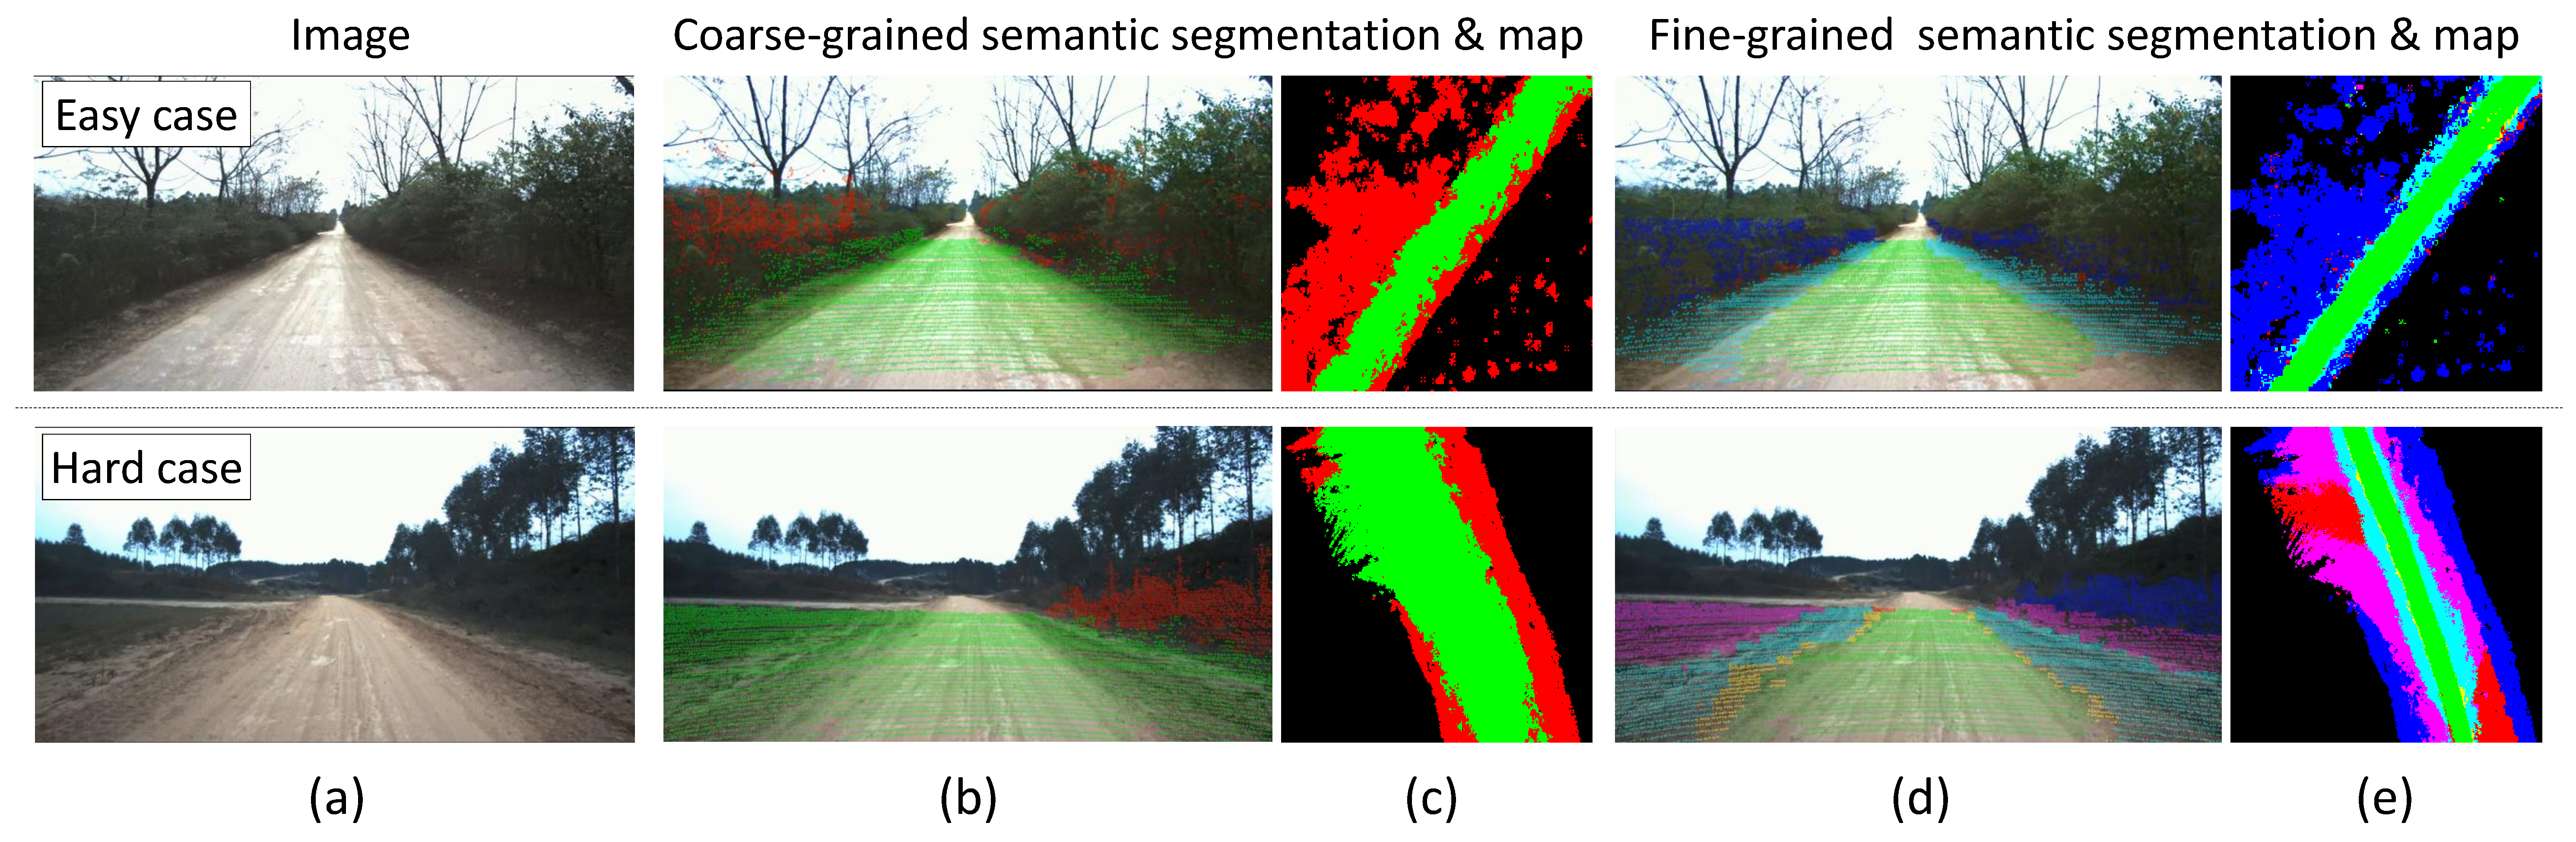
\includegraphics[width=0.95\textwidth]{problem_def.pdf}
				\vspace{-2mm}
				\captionof{figure}{The significance of fine-grained semantic segmentation and mapping in off-road environment, where coarse-grained results can hardly adapt diverse scenes. (a) scene image. (b) coarse-grained semantic segmentation (binary classification). (c) coarse-grained semantic map. (d) fine-grained semantic segmentation. (e) fine-grained semantic map.}
				\label{fig:problem_def}
			\end{center}
		}]
	}
	
	\maketitle
	%\thispagestyle{empty}
	%\pagestyle{empty}
	
	
	%%%%%%%%%%%%%%%%%%%%%%%%%%%%%%%%%%%%%%%%%%%%%%%%%%%%%%%%%%%%%%%%%%%%%%%%%%%%%%%%
	
\begin{abstract}
Road detection or traversability analysis has been a key technique for a mobile robot to traverse complex off-road scenes.
The problem has been mainly formulated in early works as a binary classification one, e.g. associating pixels with road or non-road labels.
Whereas understanding scenes with fine-grained labels are needed for off-road robots, 
as scenes are very diverse, and the various mechanical performance of off-road robots may lead to different definitions of safe regions to traverse.
How to define and annotate fine-grained labels to achieve meaningful scene understanding for a robot to
traverse off-road is still an open question.
This research proposes a contrastive learning based method. 
With a set of human-annotated anchor patches, a feature representation is learned to discriminate regions with different traversability, 
a method of fine-grained semantic segmentation and mapping is subsequently developed for off-road scene understanding.
Experiments are conducted on a dataset of three driving segments that represent very diverse off-road scenes.
An \textit{anchor accuracy} of 89.8\% is achieved by evaluating the matching with human-annotated image patches in cross-scene validation.
Examined by associated 3D LiDAR data, the fine-grained segments of visual images are demonstrated to have different levels of toughness and terrain elevation, which represents their semantical meaningfulness.
The resultant maps contain both fine-grained labels and confidence values, providing rich information to support a robot traversing complex off-road scenes.
	
	
\end{abstract}
	
	%%%%%%%%%%%%%%%%%%%%%%%%%%%%%%%%%%%%%%%%%%%%%%%%%%%%%%%%%%%%%%%%%%%%%%%%%%%%%%%%
	\section{Introduction}
	%近年来,无人驾驶技术迅猛发展。驾驶场景的语义理解,是无人车进行有效决策规划和自主行驶的前提。目前,面向城市场景的语义理解研究非常丰富。然而,越野场景以自然物体为主、缺少结构化特征的属性,使得这一问题的定义不够明确。
	Mobile robotic and autonomous driving techniques have been witnessed with tremendous progress in recent years~\cite{feng2020deep}. Driving scene understanding plays a vital role as a prerequisite for the decision making and planning of a robot to traverse in complex environments~\cite{badue2020self}.
	Nowadays researches are mainly oriented to the applications at structural scenes such as indoor, parking lots, urban streets, highways, etc.~\cite{siam2017deep},
	whereas research on understanding off-road environments is rare.
	The off-road environment is unstructured, dominated by natural objects, lacking artificial features, and its terrain conditions are various and complex.
	One of the fundamental techniques of an off-road robot is to detect safe regions (hereinafter called {\it off-road}) to traverse, which has also been termed as traversable surface~\cite{zhou2012self}, drivable corridor~\cite{nefian2006detection}, etc., in literature.
	Comparing with the roads in structured environments, where functional attributes are clearly defined by artificial features such as pavement, barrier, and markings,
	off-roads are ill-defined~\cite{ososinski2015automatic}. 
	
	Early methods of off-road detection are usually developed by assuming color, texture, boundaries of the target, where rule-based methods of extracting vanishing point and subsequently road boundaries~\cite{kong2009vanishing}\cite{shi2015fast}, and segmentation-based methods of extracting continuous regions based on certain road models are developed~\cite{alon2006off}\cite{wang2009unstructured}.
	These methods are called {\it coarse-grained} ones as the problem is formulated as a binary classification, e.g. labeling each image pixel to {\it road} or {\it non-road}.
	As illustrated in Fig. \ref{fig:problem_def}(b-c), such methods may fail to detect any region to traverse at tough terrains or extract too wide regions that lack efficiency in promoting the best choice at open area.
	Moreover, the mechanical performance of off-road robots can be very different, leading to different definitions and selections of safe regions to traverse.
	Understanding scenes with fine-grained labels is needed for off-road robots~\cite{wellhausen2019should}.
	On the other hand, deep learning methods have been studied in recent years~\cite{rateke2019passive}. 
	Semantic segmentation using deep learning techniques infers scenes at pixel- or point-levels~\cite{long2015fully}, where large-scale datasets such as Cityscapes~\cite{cordts2016cityscapes}, SemanticKITTI~\cite{behley2019semantickitti} with fine-grained labels and massive annotations are needed.
	There is no such dataset at off-road scenes. How to define and annotate fine-grained labels to achieve meaningful scene understanding for a robot to traverse off-road is still an open question.  
	
	This research proposes a contrastive learning method to achieve fine-grained semantic segmentation and mapping of off-road scenes as shown in Fig. \ref{fig:problem_def}(d-e).
	It is difficult to define fine-grained categories that are generalized at diverse off-road scenes and it is further hard for a human operator to assign fine-grained labels to each image pixel, where the definitions could be very ambiguous at natural scenes. However, it is not difficult for a human operator to annotate images by sparse anchor patches as illustrated in Fig. \ref{fig:pipeline} to indicate the regions with different semantic attributes on their traversability. Inspired by impressive progress and promising results of contrastive learning~\cite{oord2018CPC}\cite{chen2020simple}\cite{he2020momentum}, this research learns a feature representation to discriminate regions with different semantic attributes using contrastive learning, which is used to develop a method of fine-grained semantic segmentation and mapping for off-road applications.
	An off-road dataset is developed containing over 12000 image frames of three driving segments that represent very diverse off-road scenes.
	With no more than 100 training frames in all experimental settings, the test results in cross-scene validation show an 89.8\% \textit{anchor accuracy}, which is a new metric introduced to evaluate the matching with human-annotated image patches. 
	Examined by additionally measured 3D LiDAR data, 
	it is found that the fine-grained segments of visual images are semantically meaningful to represent different levels of toughness and terrain elevation.
	The resultant maps contain both fine-grained labels and confidence values, providing rich information to support a robot traversing complex off-road environments.
	
	
	%本文结构如下…
	This paper is organized as follows. First, the related works
	are introduced in Section~\ref{related_works}. Section~\ref{methodology} presents the proposed methodology in detail. Section~\ref{exp} shows experimental results. Finally, we draw conclusions in Section~\ref{conclusions}.
	
	\section{Related Works} \label{related_works}
	\subsection{Rule/Segmentation-based Methods}
	Rule/segmentation-based methods are mainly developed by assuming color, texture, boundaries of the target region, and these researches are mostly coarse-grained understanding that formulates the problem as a binary classification. They can be broadly divided into rule-based and segmentation-based methods.
	
	%Rule-based: 消失点, 三角形/梯形;
	Some rule-based methods utilize global priors like vanishing point~\cite{kong2009vanishing}\cite{shi2015fast}, which primarily depend on edge cues to obtain road area. The others assume the road region as geometric triangular~\cite{zhou2010self} or trapezoidal~\cite{jeong2002vision} shape.
	%trapezoidal\cite{ososinski2015automatic}
	
	%Segmentation-based: AdaBoost, SVM, GMM
	Segmentation-based methods formulate the problem as pixel-level segmentation tasks. Some studies~\cite{lu2014hierarchical}
	assume the region at bottom of images as road data or collect vehicle trajectories as drivable area~\cite{mei2017scene}, then label similar regions as roads.
	Other methods~\cite{alon2006off}\cite{wang2009unstructured} depend on fixed road models and make use of hybrid features to extract continuous regions.
	
	\subsection{Deep Learning Methods}
	%得益于大规模数据集的发展,深度学习的方法可以细粒度语义分割,但主要都是城市环境
	Benefit by developments of deep networks~\cite{long2015fully} and large-scale datasets with fine-grained labels like Cityscapes~\cite{cordts2016cityscapes} and SemanticKITTI~\cite{behley2019semantickitti}, deep learning methods are able to get fine-grained semantic segmentation or maps. However, most existing datasets and studies are designed for urban scenes, and research in off-road environments is still limited.
	
	%减少数据标注需求的尝试(尤其是越野场景)IV-19等
	Due to the lack of datasets, studies for off-road scenes attempt several ways to reduce the demand for fine-annotated data, such as weakly and semi-supervised learning~\cite{suger2015traversability}\cite{gao2019off}, and transfer learning~\cite{holder2016road}\cite{sharma2019semantic}. 
	One mainstream idea is automatically generating training data from other sensor modalities, such as 3D LiDAR data~\cite{gao2019off}\cite{tang2017one}, audio features~\cite{zurn2020self} and force-torque signals~\cite{wellhausen2019should}.
	Another idea is to transfer knowledge of deep networks from existing urban datasets~\cite{holder2016road} or synthetic data~\cite{sharma2019semantic} to off-road environments.
	Nevertheless, transferred models still need some fine-annotated data for finetuning, and the performance is limited by domain gaps. Meanwhile, labels from other modalities or synthetic data are too limited to support fine-grained semantic segmentation and mapping.
	
	\subsection{Contrastive Learning}
	Recent progress in contrastive learning~\cite{oord2018CPC}\cite{chen2020simple}\cite{he2020momentum} demonstrates that discriminative representations could be learned through a self-supervised pipeline, by contrasting positive and negative samples. Various sample definitions make contrastive learning suitable for diverse domains like natural language~\cite{oord2018CPC} and images~\cite{tian2019contrastive}. 
	Zhao et al.~\cite{zhao2020contrastive} introduce contrastive learning to semantic segmentation task, but rely on pixel-level labeled data for initial contrastive learning and generating pseudo labels for unlabeled images.
	
	Inspired by the promising results of contrastive learning, but different from settings in~\cite{zhao2020contrastive}, this work only relies on a small number of sparse anchor annotations without pixel-level labels to learn feature representations to discriminate regions with different semantic attributes, which is further used to develop a method of fine-grained semantic segmentation and mapping.
	
	\begin{figure*}[]
		%	\vspace{-2mm}
		\centering
		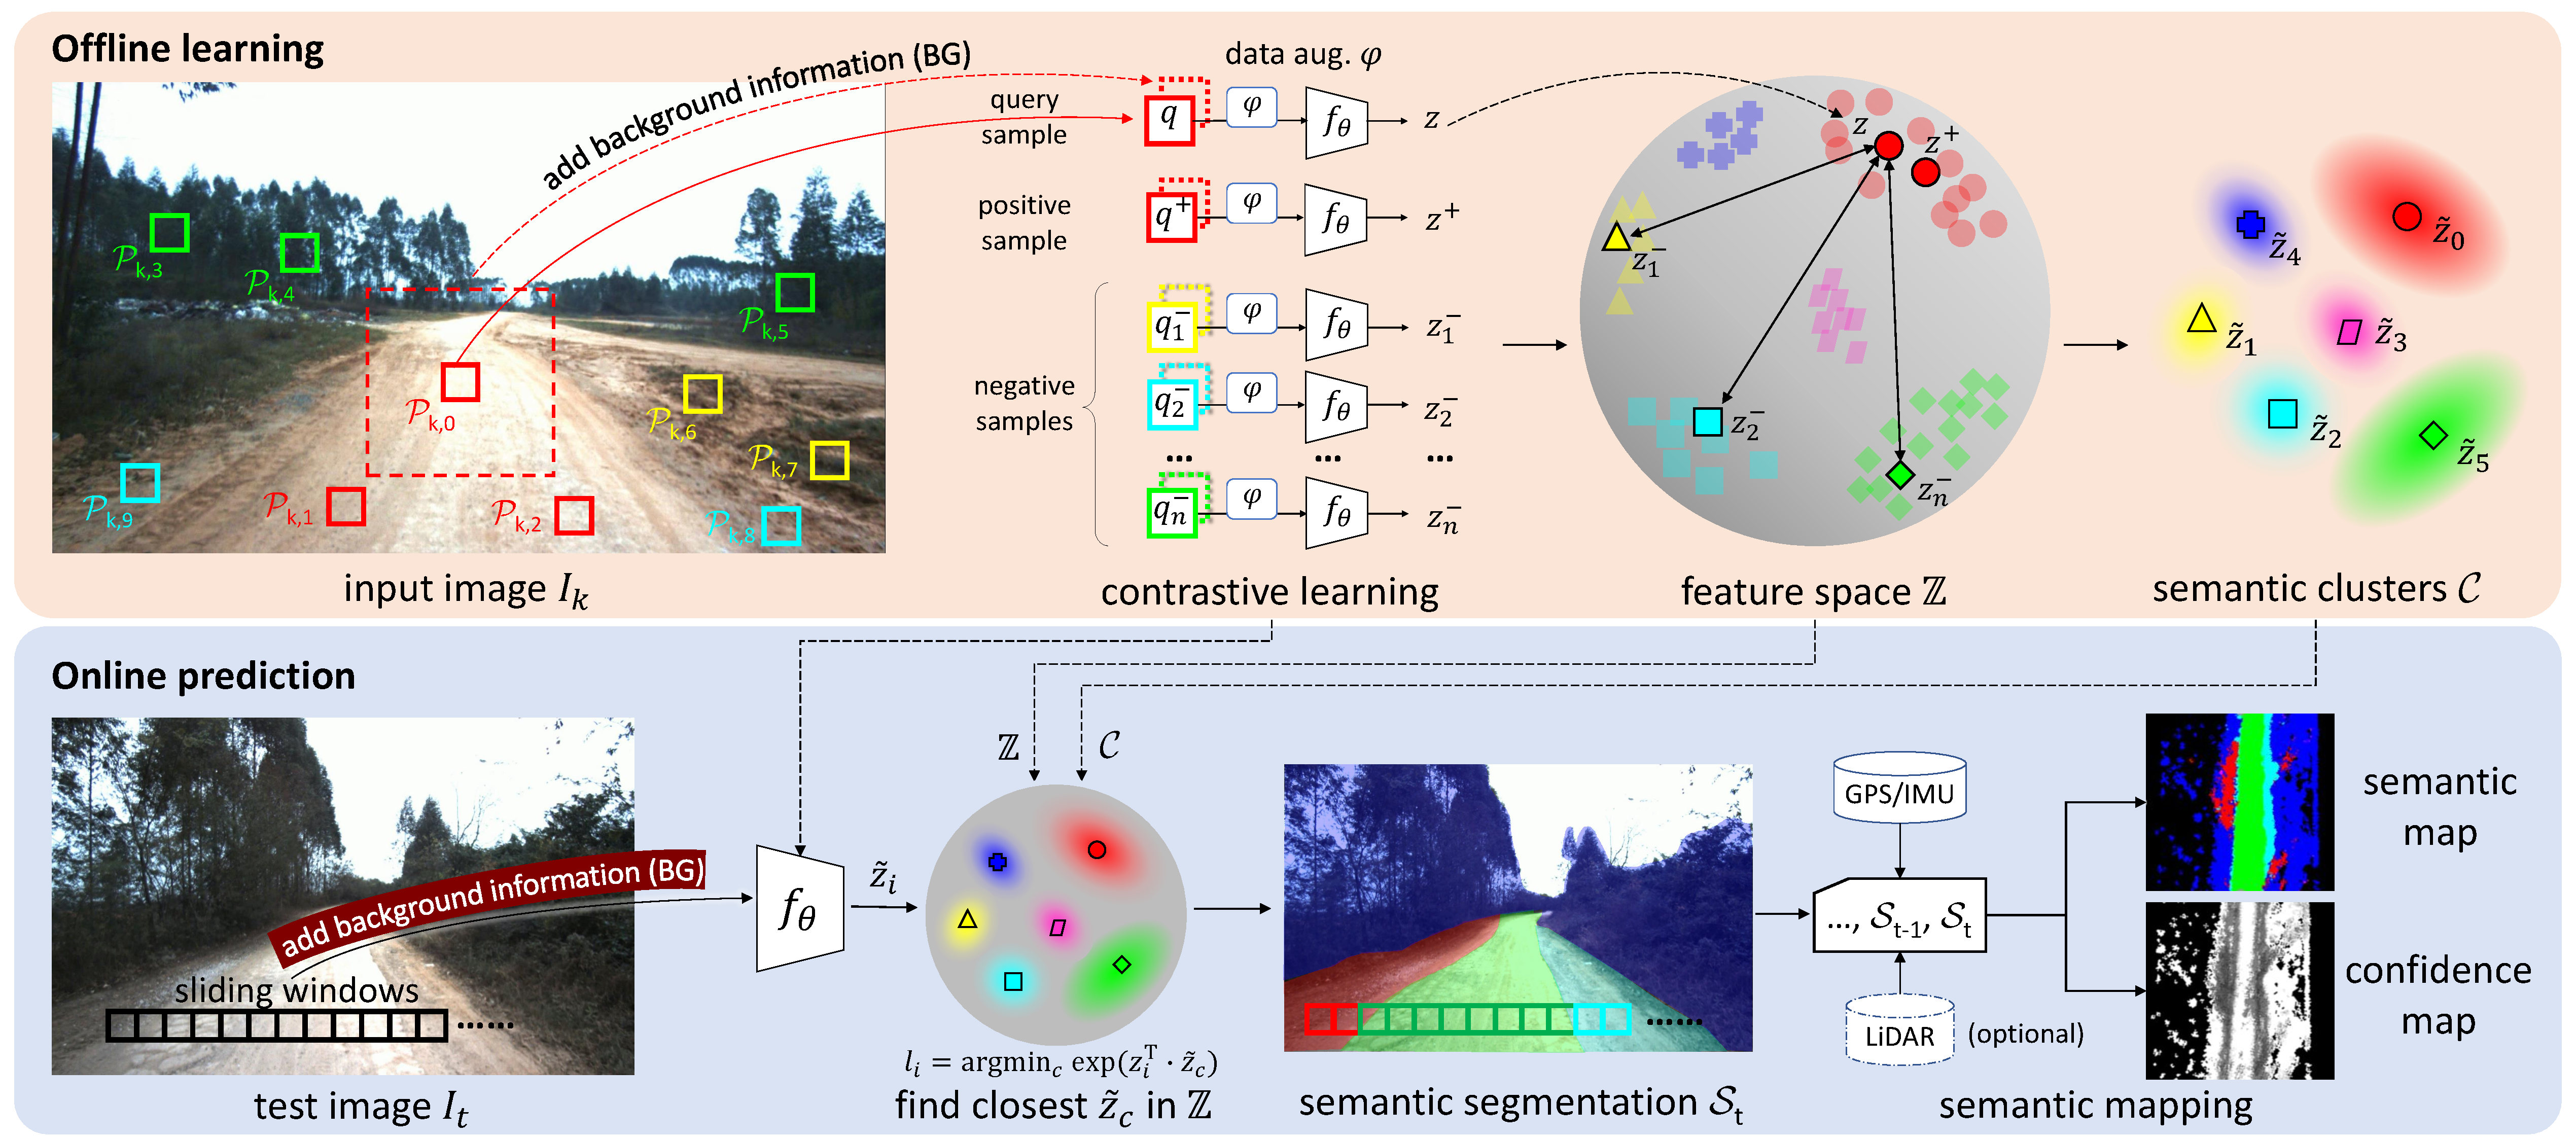
\includegraphics[width=\textwidth]{pipeline.pdf}
		\caption{The proposed pipeline for fine-grained off-road semantic segmentation and mapping via contrastive learning.}
		\label{fig:pipeline}
		\vspace{-2mm}
	\end{figure*}
	
	\section{Methodology} \label{methodology}
	
	\subsection{Problem Formulation}
	
	A training image $I_k$ has a number of anchor patches $A_k=\{\mathcal{P}_{k,i}=<p_{k,i},a_{k,i}>\}$, where an anchor patch $\mathcal{P}_{k,i}$ is a pair of an image patch $p_{k,i}$ and a label $a_{k,i}$. Here, $a_{k,i}$ has no semantic meaning, but is an identifier of the image patches with similar or different semantic properties.
	Let $z=f_{\theta}(p)$ be an encoder converting a high-dimensional image patch $p$ to a normalized low-dimensional feature vector $z\in \mathbb{Z}^D$. 
	We use exponential cosine similarity $sim(p_i,p_j)=exp(z_i^T \cdot z_j)$ to measure the similarity of two image patches via their low-dimensional feature vectors.
	Therefore, given an anchor patch $\mathcal{P}_{k,i}$, its similarity to another anchor patch $\mathcal{P}_{k,j}$, i.e. $sim(p_{k,i},p_{k,j})$, should be higher if they share the same label $a_{k,i}=a_{k,j}$, whereas lower if the labels are different $a_{k,i} \neq a_{k,j}$.
	In order to make the annotation operational easy, in this research, the labels of the anchor patches are comparable only if they belong to the same image.
	
	Given a set of training images $\mathcal{I}=\{I_k\}$ with anchor patches $\mathcal{A}=\{A_k\}$ on each of them, this research is to find a representation $f_{\theta}$ that encodes image patch $p$ to $z$, where at the low-dimensional feature space $\mathbb{Z}^D$, the $z$ of similar semantic meaning distribute closely. 
	This research finds $f_{\theta}$ through contrastive learning, which is further used in an application of fine-grained semantic segmentation and mapping for off-road traversability analysis.
	
	\begin{figure}[]
		\centering
		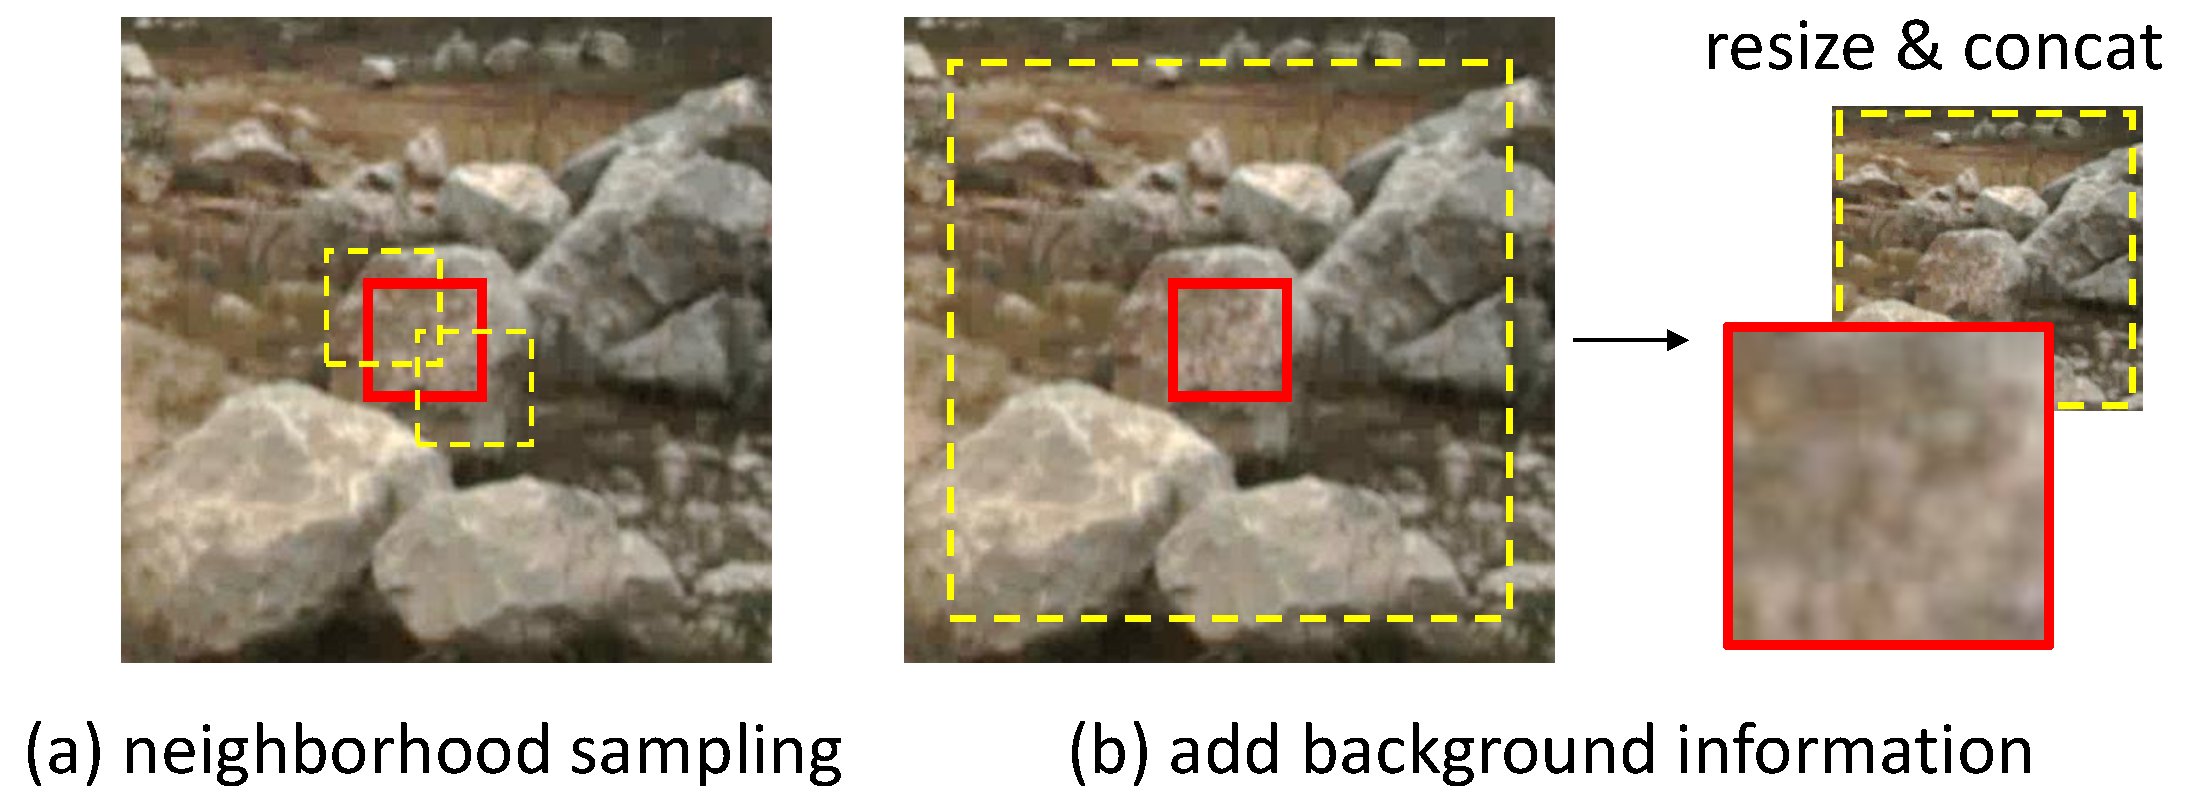
\includegraphics[scale=0.23]{dataaug.pdf}
		\caption{Illustration of (a) neighborhood sampling strategy, and (b) how to add background information with the foreground image patch.}
		\label{fig:dataaug}
	\end{figure}
	
	\subsection{Feature Representation through Contrastive Learning}
	
	\subsubsection {Sampling Strategy}
	
	In each training step, an anchor patch $\mathcal{P}_{k,i}$ is selected to compose a query sample $q$, then a positive sample $q^+$ and $n$ negative samples $\{q^-_i|i=1,..,n\}$ are subsequently composed on the anchor patches of the same image $I_k$.
	
	Based on the label $a_{k,i}$ of $\mathcal{P}_{k,i}$, the anchor patches in the same image $I_k$ are divided into two sets, where $\{\mathcal{P}_{k,i}^+\}$ denotes those sharing the same label $a_{k,i}$, whereas $\{\mathcal{P}_{k,i}^-\}$ for the rest.
	Assume that an off-road scene is spatially continuous, i.e. nearby regions could be semantically similar. An anchor patch $p$ is first randomly selected from $\{\mathcal{P}_{k,i}^+\}$, where an image patch is randomly clipped from $p$'s neighborhood to compose a positive sample $q^+$. As illustrated in Fig.~\ref{fig:dataaug}(a), the randomly clipped neighborhood patches should have the center points within the original one. Similarly, $n$ negative samples $\{q^-_i\}$ are composed on $\{\mathcal{P}_{k,i}^-\}$.
	
	\subsubsection{Composing Sample Data}
	
	As shown in Fig.~\ref{fig:dataaug}(b), sample data contains foreground and background image patches to describe both local and global features. The foreground is image patch $p$, while the background is centered at $p$ but with a larger region to provide global scene context. The foreground and background patches are firstly resized to the same scale, then concatenated along the channel dimension to compose a 6-channel tensor.
	With an image patch $p$, sample data is composed in the same way for the query, positive and negative samples.
	
	In order to improve robustness in diverse scenes, data augmentation (denoted by $\varphi$ in Fig.~\ref{fig:pipeline}) is conducted on the 6-channel tensor of each sample data before forwarding it to the network of $f_{\theta}$. In this research, data augmentation includes random flip, random greyscale, and color jitter, which randomly changes the brightness, contrast, and saturation of an image.
	
	\subsubsection{Network Design and Loss Function}
	A CNN backbone network in practical terms, i.e. AlexNet~\cite{krizhevsky2012imagenet} is used to model $f_{\theta}$, which converts the 6-channel tensor of a query, positive or negative sample to a normalized low-dimensional feature vector $z\in \mathbb{Z}^D$.
	Contrastive learning is used to find $\theta$ in $f_{\theta}$, with which the exponential cosine similarity of the $z$ are high if they share the same labels, whereas low for those differences.
	Following the principle of previous contrastive learning studies~\cite{he2020momentum}, a contrastive loss function InfoNCE~\cite{oord2018representation} is implemented:
	
%	\vspace{-2mm}
	\begin{equation}\label{loss}
	L=-\log {\dfrac{\exp (z^T \cdot z^+/\tau)}{\exp (z^T \cdot z^+/\tau)+\sum_{i=1}^{n}{\exp (z^T \cdot z_i^-/\tau)}}}
	\end{equation}
	where $\tau$ denotes a temperature hyper-parameter.
	
	In this work, since the positive and negative samples are comparable only in the same image, the limited quantity makes it possible to get feature representations with reasonable memory consumption. In practice, unlike the typical contrastive learning studies~\cite{Wu_2018_CVPR} using a memory bank to store feature vectors for each training sample, we randomly select positive/negative samples and calculate their features at each training step.
	
	\subsection{Off-road Semantic Segmentation and Mapping}
	
	As illustrated in Fig.~\ref{fig:pipeline}, the workflow contains offline learning and online prediction, while the latter is composed of further two steps: semantic segmentation of single images and semantic mapping using multiple images.
	
	\subsubsection{Offline Learning}
	Given a set of training images $\mathcal{I}=\{I_k\}$ with anchor patches $\mathcal{A}=\{A_k\}$ on each of them, a feature encoder $f_\theta$ is thus learned to convert each image patch to a normalized low-dimensional vector $z\in \mathbb{Z}^D$ in the space of $\mathbb{Z}^D$, the image patches with the same labels are projected close, whereas far for the others.
	
	The $z$ of the anchor patches are then clustered by the K-means method, where a set of mean points $\mathcal{C}=\{\tilde{z}_c\}$ are extracted, representing the features of $\mathcal{K}$ dominant semantic clusters. Here, clustering number $\mathcal{K}$ is a hyper-parameter, which decides the granularity of semantic segmentation.
	
	\subsubsection{Semantic Segmentation}
	
	Given the current image $\mathcal{I}_t$, semantic segmentation $\mathcal{S}_t$ is conducted by generating image patches using sliding windows and predicting a semantic label for each image patch.
	Given an image patch $p_i$, a semantic label is predicted as follows. A 6-channel tensor data is first composed, containing both local and global features of the image patch. The data is then projected by $f_{\theta}$ to a normalized lower-dimensional feature vector $z_i$, which is subsequently compared with the set of feature vectors $\mathcal{C}=\{\tilde{z}_c\}$ representing the $\mathcal{K}$ dominant semantic labels. The image patch is assigned as the semantic label $l_i$ that has the best match on its feature vector, i.e. $l_i = \arg\min_c exp(z_i^T \cdot \tilde{z}_c)$.
	
	To make up denser semantic segmentation, we could adjust the step size of sliding windows. For example, we can assign the semantic label to $3*3$ pixels centered at each image patch, while setting sliding windows' horizontal/vertical step size to 3 pixels, then get denser semantic segmentation results.
	
	\subsubsection{Semantic Mapping} \label{3_SM}
	
	Centered at the ego vehicle's location at the frame, a horizontal plane is drawn at the ground level and tessellated into regular grids.  
	The pixel labels of the current image can be projected onto the grids with the camera’s calibration parameters. 
	Besides, the pixel labels of early frames can also be projected onto the grids with additionally the vehicle's localization data at each frame.
	If a 3D LiDAR is associated, the projection can be conducted via LiDAR points, where the up and down of off-road terrain can be taken into calculation. 
	Since a single grid can have multiple label predictions, let $\sigma_{x,y}^c$ denote the counts of predicting label $c$ of grid $(x,y)$, the semantic label $l_{x,y}=\mathop{\text{argmax}_{c} (\sigma_{x,y}^c)}$ is assigned to the grid. Meanwhile, a confidence map is estimated to indicate the confidence of predicted labels. The confidence value of grid $(x,y)$ is assigned as $\max(\sigma_{x,y}^c)/\sum{\sigma_{x,y}^c}$, which can also serve as a measure to evaluate prediction consistency.
	
	\section{Experimental Results}	\label{exp}
	\subsection{Experimental Data}
	An off-road dataset is developed to evaluate the proposed method.
	The dataset is collected by an instrumented vehicle with a front-view monocular RGB camera,
	a GPS/IMU suite, and a 3D LiDAR. In this work, we use visual images for semantic segmentation, 
	while GPS/IMU provides 6 DoF poses of the ego vehicle, which is used for mapping. 
	3D LiDAR is mainly used to examine the semantic meaning of the fine-grained segmentation, 
	while it is also used in this research in projecting visual labels to a horizontal plane so as to generate a more accurate map by considering the up and down of off-road terrain.
	
	\begin{table}[]
		\centering
		%	\renewcommand{\arraystretch}{1.2}
		\caption{Statistics of the off-road dataset}
		\label{tab:dataset}
		\begin{tabular}{cccc} 
			\hline
			& subset A & subset B & subset C  \\ 
			\hline
			total frames        & 5064     & 3239     & 4098      \\
			frames for training & 50       & 100      & 80        \\
			anchors       & 973      & 1606     & 1437      \\
			\hline
		\end{tabular}
	\end{table}
	
	\begin{figure}[]
		%	\vspace{-2mm}
		\centering
		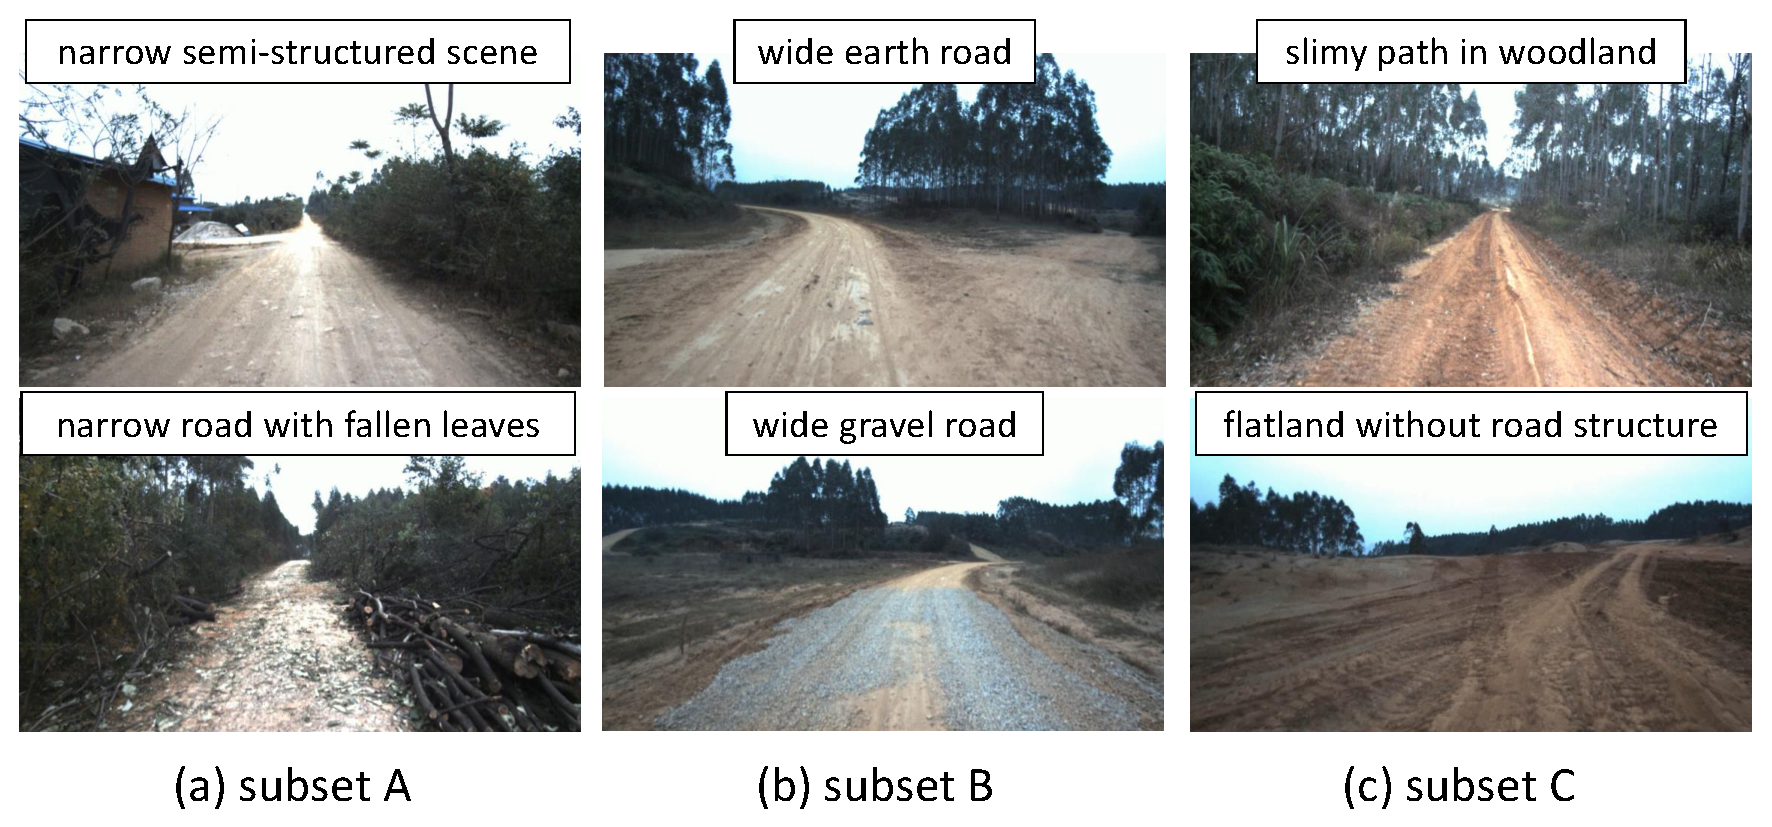
\includegraphics[scale=0.28]{dataset.pdf}
		\caption{Typical scenes in three sub-datasets, which include diverse off-road scenarios.}
		\label{fig:dataset}
	\end{figure}
	
	As shown in Table~\ref{tab:dataset}, the dataset contains over 12000 image frames of three driving segments that represent very diverse off-road scenes.
	Take subset A as an example, 50 image frames are randomly selected, which account for 10\% of the total 5064 frames of subset A. 
	973 anchor patches are annotated on the 50 image frames by a human operator, which are used in training.
	The rest image frames of subset A are used in testing, 
	and the image frames of subset B and C are also used to test the model trained on subset A in the experiment of cross-scene validation.
	Experiments on subset B and C are conducted in the same way to examine the results of semantic segmentation.
	To this end, image frames are used for testing and image patches are manually annotated in the same way as the anchors, which are used as \textit{ground truth} to evaluate the accuracy of the results.
	
	The three subsets contain driving data at very different off-road scenes. 
	As illustrated in Fig.~\ref{fig:dataset}, the scenarios in
	subset A are mostly narrow roads with bushes aside, subset B are relatively wide scenes, and subset C includes diverse
	scenarios like slimy paths in woodland and flatland without
	road structure. In the experiments, we train and test the
	proposed method on different subsets to evaluate its cross-scene generalization performance.
	
	\subsection{Evaluation Metrics}
	
	\begin{figure*}[]
		%	\vspace{-2mm}
		\centering
		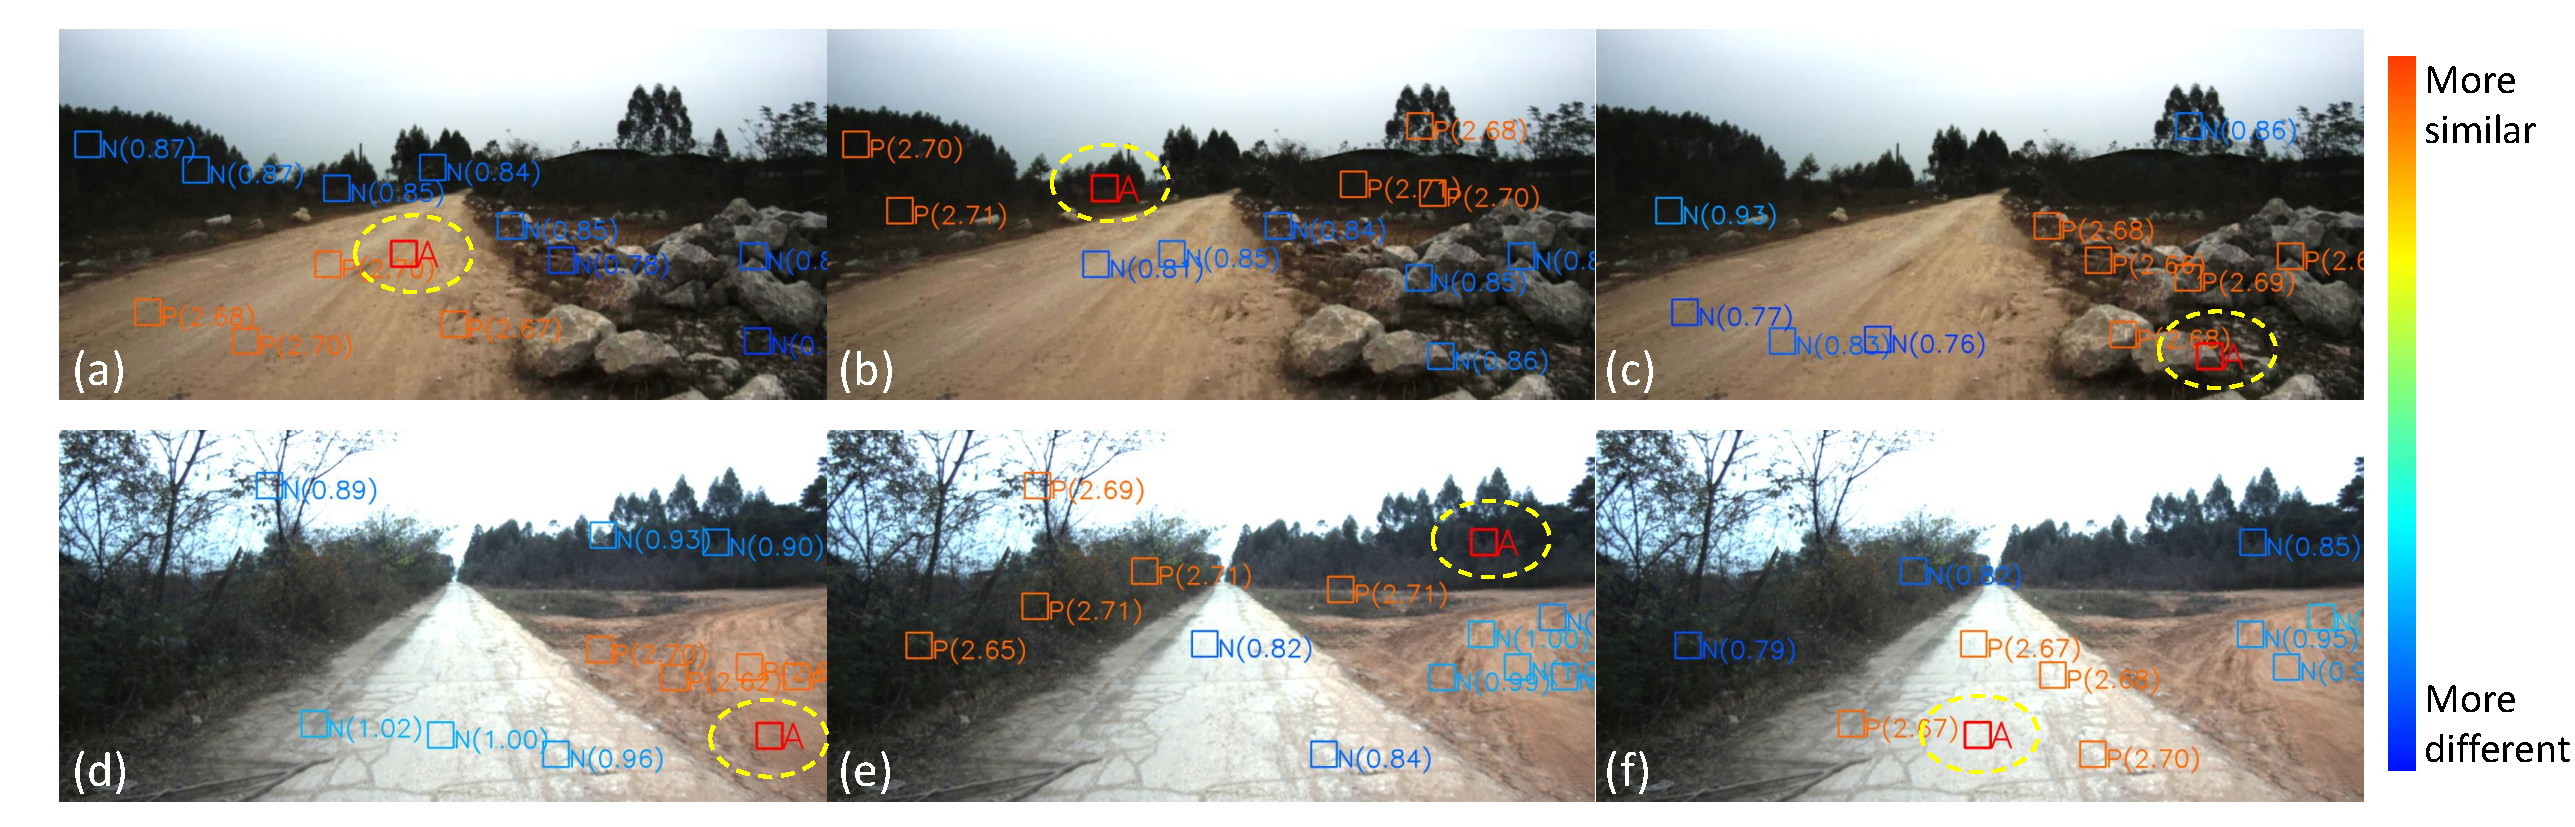
\includegraphics[width=0.9\textwidth]{anchor_dis.pdf}
		\caption{Visualization of feature similarity of query anchor (A) to its positive (P) and negative (N) samples. Query anchors are circled by yellow rings. Numbers in parentheses measure samples' exponential cosine similarity to the query anchor.}
		\label{fig:anchor_dis}
	\end{figure*}
	
	Suppose that there are $N$ anchors in one frame, then any two anchors must be either positive or negative samples of each other. Hence, there exists $N \cdot(N-1)$ pairs anchor constraints.
	%假设一帧图像中有$N$个锚点,两两互为正/负样本,则存在$N\cdot(N-1)$对正负样本约束
	We denote positive samples' constraints as $Pos(i,j)$. If anchor patch $\mathcal{P}_{k,i}$ and $\mathcal{P}_{k,j}$ are positive samples of each other and classified into the same semantic cluster, then $Pos(i,j)=1$. Otherwise, if they are not classified to the same semantic cluster, $Pos(i,j)=0$.
	Negative samples' constraints are defined in a similar way and denoted as $Neg(i,j)$.
	%正样本约束:若锚点$a_i$和$a_j$互为正样本,且聚类标签$Lab_i=Lab_j$,则满足正样本约束,并记$Pos(i,j)=1$,否则$Pos(i,j)=0$. 负样本约束$Neg(i,j)$定义同理;
	
	We use the following metrics called \textit{anchor accuracy} to evaluate how well the clustering results fit human annotations:
	\begin{equation}
	\label{R}
	\mathcal{R}=\dfrac{\sum_{i,j}{Pos(i,j)}+\sum_{i,j}{Neg(i,j)}}{N\cdot (N-1)}, ~i \neq j
	\end{equation}
	Essentially, it can be seen as Rand Index~\cite{rand1971objective}, which is a commonly used measurement for clustering.
	
	\begin{table*}
		\centering
		\caption{Cross-Scene Validation Results ($\mathcal{R}$) on Different Datasets}
		\label{tab:cross_eval}
		\renewcommand{\arraystretch}{1.2}
		\begin{threeparttable}
			\begin{tabular}{ccc|ccc|ccc|ccc!{\color{black}\vrule}c} 
				\hline
				\multirow{3}{*}{model} & \multirow{3}{*}{\makecell[c]{data\\ aug.}} & \multirow{3}{*}{\makecell[c]{BG\\ size}} & \multicolumn{3}{c|}{train on subset A}                                                                             & \multicolumn{3}{c|}{train on subset B}                                                                             & \multicolumn{3}{c|}{train on subset C}                                                                             & \multirow{3}{*}{\makecell[c]{$\bar{\mathcal{R}}$ on \\ test sets}}                      \\ 
				\cline{4-12}
				&                            &                             & \multicolumn{3}{c|}{test on}                                                                                       & \multicolumn{3}{c|}{test on}                                                                                       & \multicolumn{3}{c|}{test on}                                                                                       &                                                      \\
				&                            &                             & A      & B                                                   & C                                                   & B      & A                                                   & C                                                   & C      & A                                                   & \multicolumn{1}{c|}{B}                              &                                                      \\ 
				\hline
				base                   & $\times$                          & $\times$                           & 0.9854 & {\cellcolor[rgb]{1,0.906,0.906}}0.8548              & {\cellcolor[rgb]{0.992,0.722,0.722}}0.8509          & 0.9997 & {\cellcolor[rgb]{1,0.906,0.906}}0.7957              & {\cellcolor[rgb]{1,0.906,0.906}}0.8492              & 0.9966 & {\cellcolor[rgb]{1,0.906,0.906}}0.8288              & {\cellcolor[rgb]{0.992,0.745,0.749}}0.9258          & {\cellcolor[rgb]{1,0.906,0.906}}0.8509               \\
				base\_DA               & \checkmark                          & $\times$                          & 0.9693 & {\cellcolor[rgb]{0.996,0.773,0.773}}0.8792          & {\cellcolor[rgb]{1,0.906,0.906}}0.8422              & 0.9959 & {\cellcolor[rgb]{0.992,0.733,0.733}}0.8210          & {\cellcolor[rgb]{0.992,0.745,0.749}}0.8625          & 0.9913 & {\cellcolor[rgb]{1,0.898,0.898}}0.8296              & {\cellcolor[rgb]{1,0.906,0.906}}0.9119              & {\cellcolor[rgb]{0.996,0.835,0.835}}0.8578           \\
				BG192                  & \checkmark                          & 192                         & 0.9939 & {\cellcolor[rgb]{0.976,0.471,0.478}}0.9330          & {\cellcolor[rgb]{0.973,0.412,0.42}}\textbf{0.8650}  & 0.9994 & {\cellcolor[rgb]{0.98,0.514,0.518}}0.8524           & {\cellcolor[rgb]{0.973,0.412,0.42}}\textbf{0.8899}  & 0.9944 & {\cellcolor[rgb]{0.98,0.537,0.545}}0.8653           & {\cellcolor[rgb]{0.98,0.502,0.51}}0.9468            & {\cellcolor[rgb]{0.976,0.475,0.482}}0.8920           \\
				BG256                  & \checkmark                          & 256                         & 0.9987 & {\cellcolor[rgb]{0.976,0.455,0.463}}0.9360          & {\cellcolor[rgb]{0.976,0.463,0.471}}0.8627          & 0.9991 & {\cellcolor[rgb]{0.976,0.475,0.482}}0.8577          & {\cellcolor[rgb]{0.98,0.486,0.494}}0.8839           & 0.9934 & {\cellcolor[rgb]{0.98,0.525,0.533}}0.8665           & {\cellcolor[rgb]{0.976,0.451,0.459}}0.9512          & {\cellcolor[rgb]{0.976,0.467,0.471}}0.8930           \\
				BG320                  & \checkmark                          & 320                         & 0.9986 & {\cellcolor[rgb]{0.973,0.412,0.42}}\textbf{0.9433}  & {\cellcolor[rgb]{0.984,0.612,0.616}}0.8559          & 0.9980 & {\cellcolor[rgb]{0.973,0.412,0.42}}\textbf{0.8667}  & {\cellcolor[rgb]{0.976,0.42,0.427}}0.8895           & 0.9958 & {\cellcolor[rgb]{0.973,0.412,0.42}}\textbf{0.8776}  & {\cellcolor[rgb]{0.973,0.412,0.42}}\textbf{0.9544}  & {\cellcolor[rgb]{0.973,0.412,0.42}}\textbf{0.8979}   \\
				\hline
			\end{tabular}
			\begin{tablenotes}
				\footnotesize
				\item[*] \textbf{BG}: background; \textbf{base}: pipeline without data augmentation or background information; \textbf{base\_DA}: use data augmentation, without background information; \textbf{BG192/256/320}: complete pipeline with different background size; \textbf{$\bar{\mathcal{R}}$}: average anchor accuracy $\mathcal{R}$.
			\end{tablenotes}
		\end{threeparttable}
		\vspace{-3mm}
	\end{table*}
	
	\subsection{Results on Proposed Method}
	%说明一下三个实验设计的目的:1.探究对比学习学到的特征表达、距离度量是否有效;2.通过交叉验证说明我们设计的模型具有较优的性能和不同场景下的泛化能力;3.通过构建细粒度语义地图/置信度地图,结合case study和激光平整度统计分析,说明细粒度分类结果的有效性。
	To evaluate the proposed method, we design the following experiments: (1) feature similarity measurement, explore the validity of feature encoder and similarity measurement learned by contrastive learning. (2) cross-scene validation and ablation study, verify the performance and robustness of our proposed method in diverse test scenes while exploring the effects of different module settings. (3) fine-grained semantic segmentation and mapping, make concrete case study and statistical analysis from additional LiDAR data to show the validity of our fine-grained results.
	
	
	\begin{figure}[]
		%	\vspace{-2mm}
		\centering
		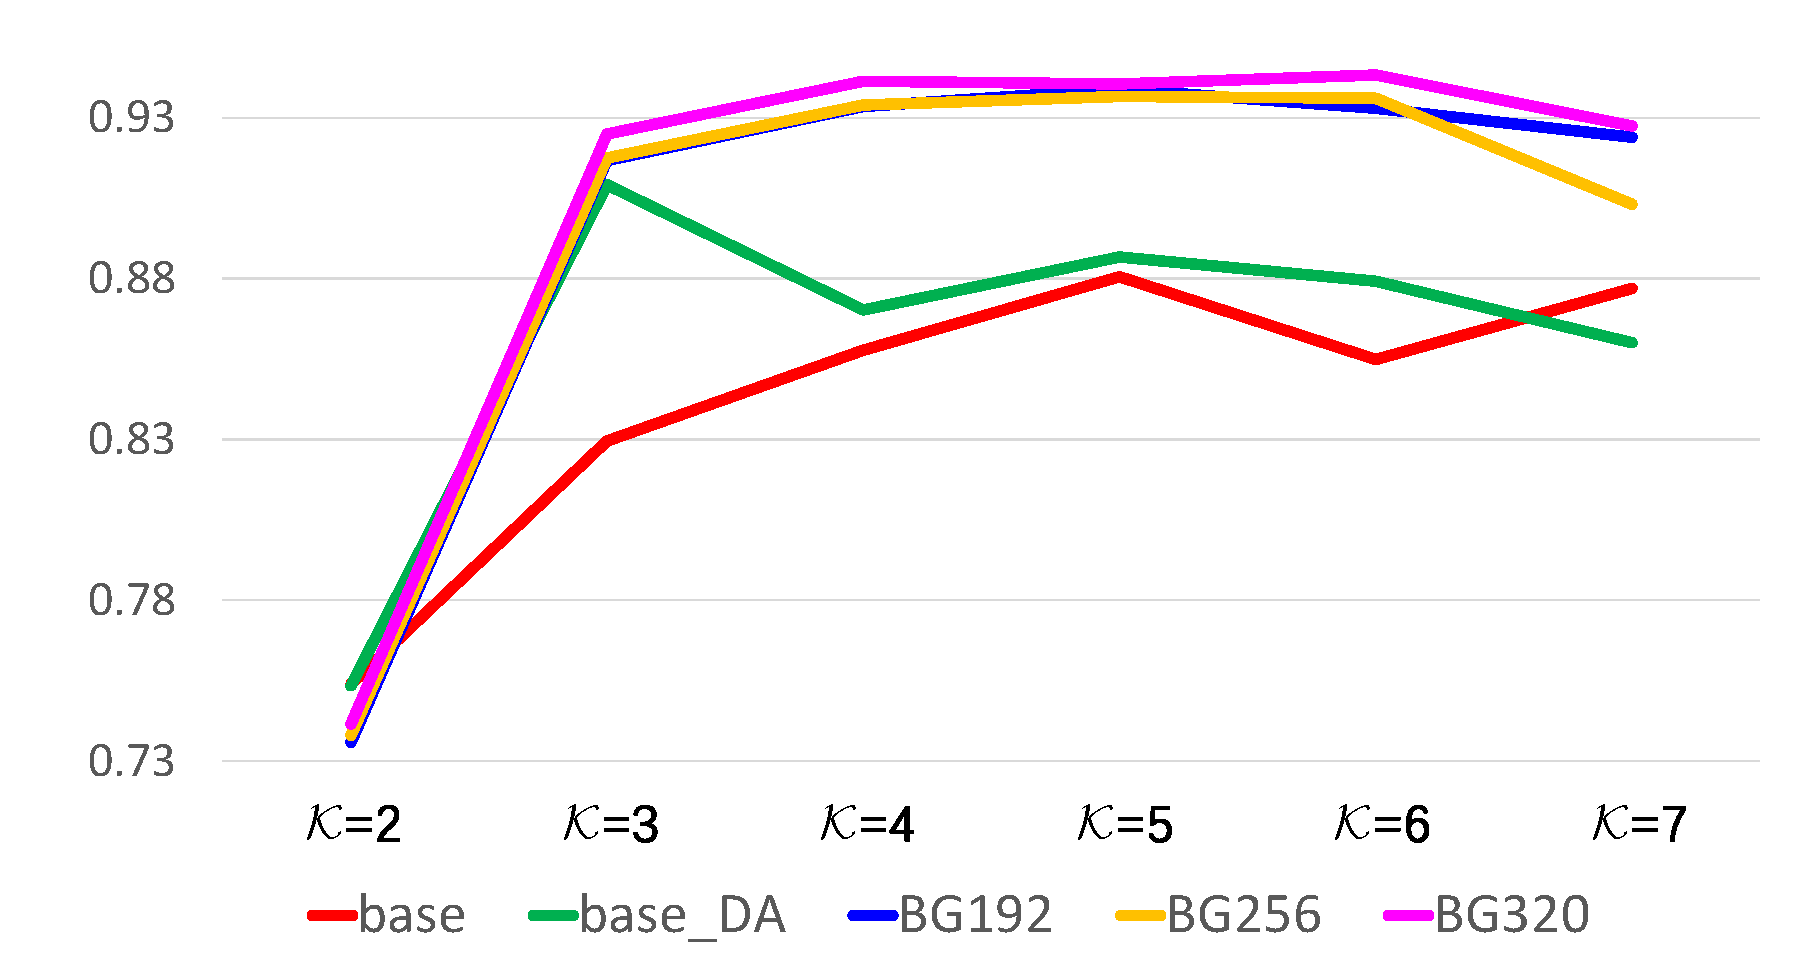
\includegraphics[scale=0.25]{kmeans_exp.pdf}
		\caption{Average $\mathcal{R}$ of models under different clustering number $\mathcal{K}$.}
		\label{fig:kmeans_exp}
	\end{figure}
	
	\subsubsection{Feature Similarity Measurement}
	%\textbf{回答问题}:对比学习模块学到的特征距离度量是否有效?\textbf{结论}:对比学习学到的特征距离度量,可以满足“语义相似的patch特征距离更近,语义不同的patch特征距离更远”的特性。
	The feature encoder $f_\theta$ aims to make similar image patches closer and different image patches farther in feature space.
	%The core module in our proposed pipeline is the feature encoder $f_\theta$, which projects a high-dimensional image patch to a low-dimensional feature vector in space $\mathbb{Z}$. Its purpose is to make feature similarity closer between similar image patches, while farther between different image patches. 
	In Fig.~\ref{fig:anchor_dis}, we visualize some concrete cases of the learned similarity measurement $sim(p_i,p_j)=exp(z_i^T \cdot z_j)$. In all images, the query anchors are circled by yellow rings, while the other anchor patches are randomly sampled and colorized by their exponential cosine similarity to the query anchor. For example, in Fig.~\ref{fig:dataaug}(a), the query anchor is located on the earth road. We can find that patches on the earth road are closer to red, and other patches located on different semantic areas are generally blue, which indicates the lower similarity to the query anchor. The feature similarity distribution is in accord with the semantic differences. Similar situations are general in other images. \textbf{As a result, the feature encoder and similarity measurement learned by contrastive learning are able to distinguish similar or different image patches.}
	
	\subsubsection{Cross-Scene Validation and Ablation Study}
	
	%\textbf{问题1}:我们的模型设计(数据增强+背景信息)是否性能较优,且在不同条件下有泛化能力?
	%\textbf{结论1}:从表\ref{tab:cross_eval}中最后一列看出,BG320模型在测试集上具有最好的准确率;且加入了背景信息的3个模型在训练/测试集不同的情况下都可以达到0.85以上的准确率(泛化能力)。 说明我们的模型设计性能较优且有一定泛化能力。
	%
	%\textbf{问题2}:[Ablation Study 1]数据增强、背景信息分别起到了多少作用?
	%\textbf{结论2}:从表\ref{tab:cross_eval}可以看出数据增强和背景信息都有作用,添加背景带来的性能提升更大;背景尺寸的增加带来略微提升,不显著;
	%
	%\textbf{问题3}:[Ablation Study 2]聚类数量K对结果的影响如何?
	%\textbf{结论3}:从图\ref{fig:kmeans_exp}看出,聚类数量的变化会略微影响锚点吻合度, 但不是决定因素。整体来看,不同模型的性能排序与结论1一致。
	For comprehensive evaluations of the proposed method, we make cross-scene validation on models with different settings, and the statistics are shown in Table~\ref{tab:cross_eval}. The table cells are colorized along column data when training and testing on different subsets. The last column lists the average anchor accuracy $\bar{\mathcal{R}}$ on test sets (the subsets different with the training one). It is obvious that \textit{BG320} has the best performance on test sets, and all three models with background information have $\mathcal{R}$ over 85\% among all conditions, which demonstrates the robustness of our proposed method.
	The data augmentation and background information can both increase models' performance, while the latter makes more contribution. Increasing background size could sightly improve overall performance, but is not obvious in all situations.
	
	\begin{figure*}[]
		%	\vspace{-2mm}
		\centering
		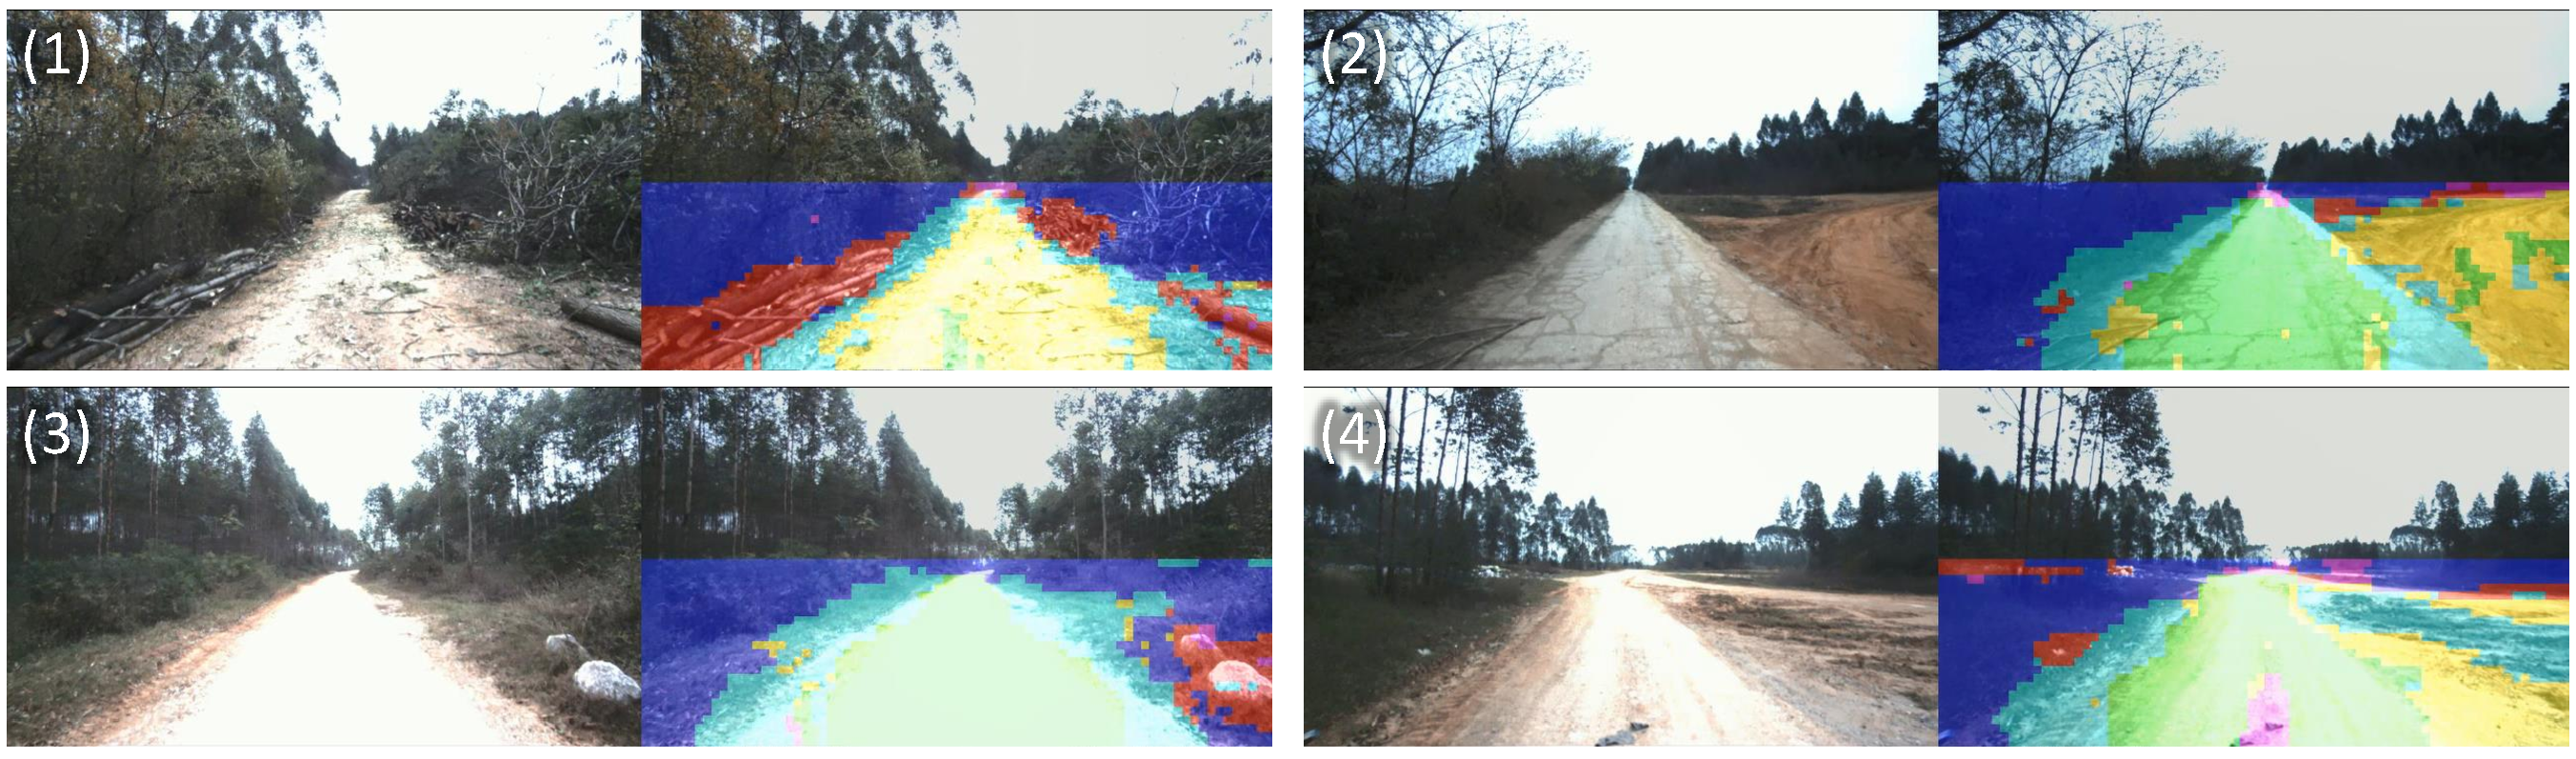
\includegraphics[width=0.88\textwidth]{semantic_segmentation.pdf}
		\caption{Some results of fine-grained semantic segmentation.}
		\label{fig:semantic_segmentation}
	\end{figure*}
	
	\begin{figure*}[]
		%	\vspace{-2mm}
		\centering
		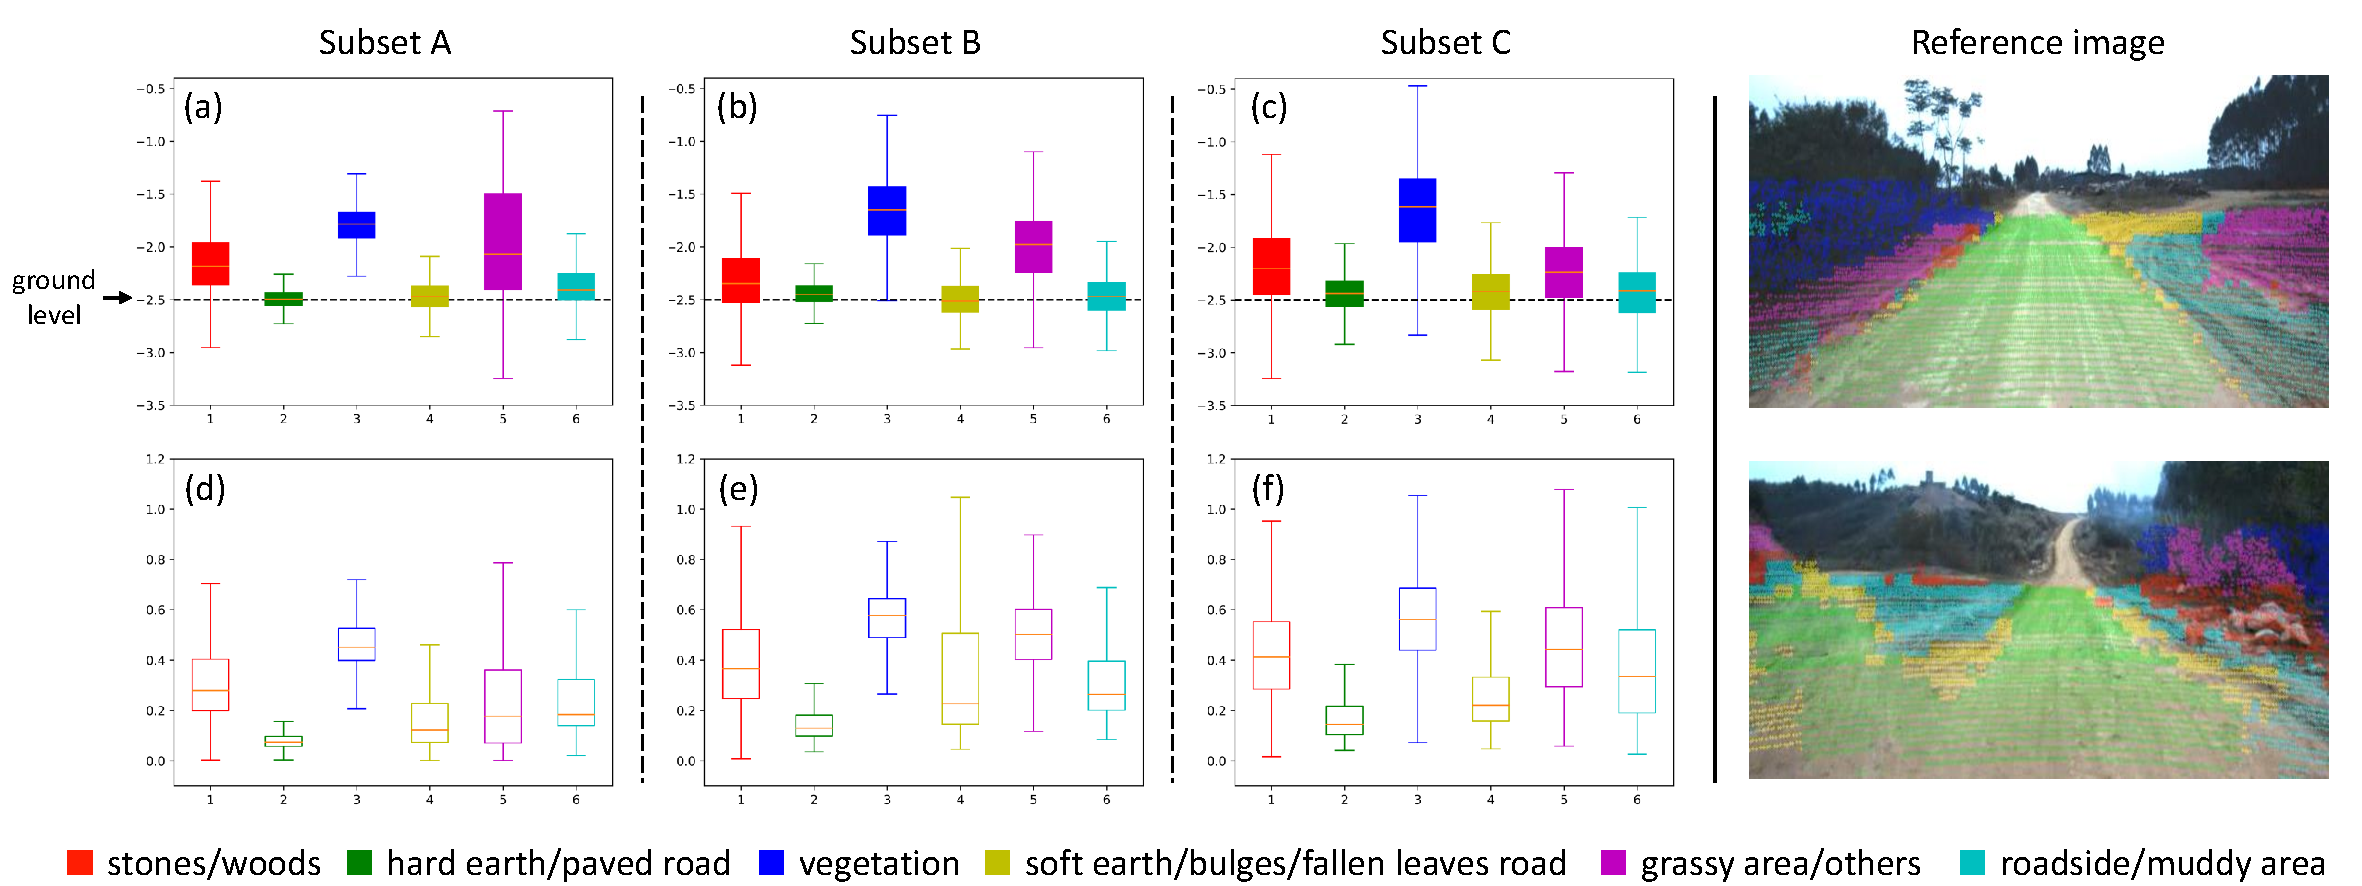
\includegraphics[width=0.95\textwidth]{lidar_analysis.pdf}
		\caption{Traversability analysis of semantic clusters by 3D LiDAR data. (a-c) boxplots of points average height, indicate height distribution of different categories. (d-f) boxplots of points height variance, indicate surface flatness and traversability cost. }
		\label{fig:lidar_analysis}
		\vspace{-5mm}
	\end{figure*}
	
	
	\begin{figure*}[]
		\centering
		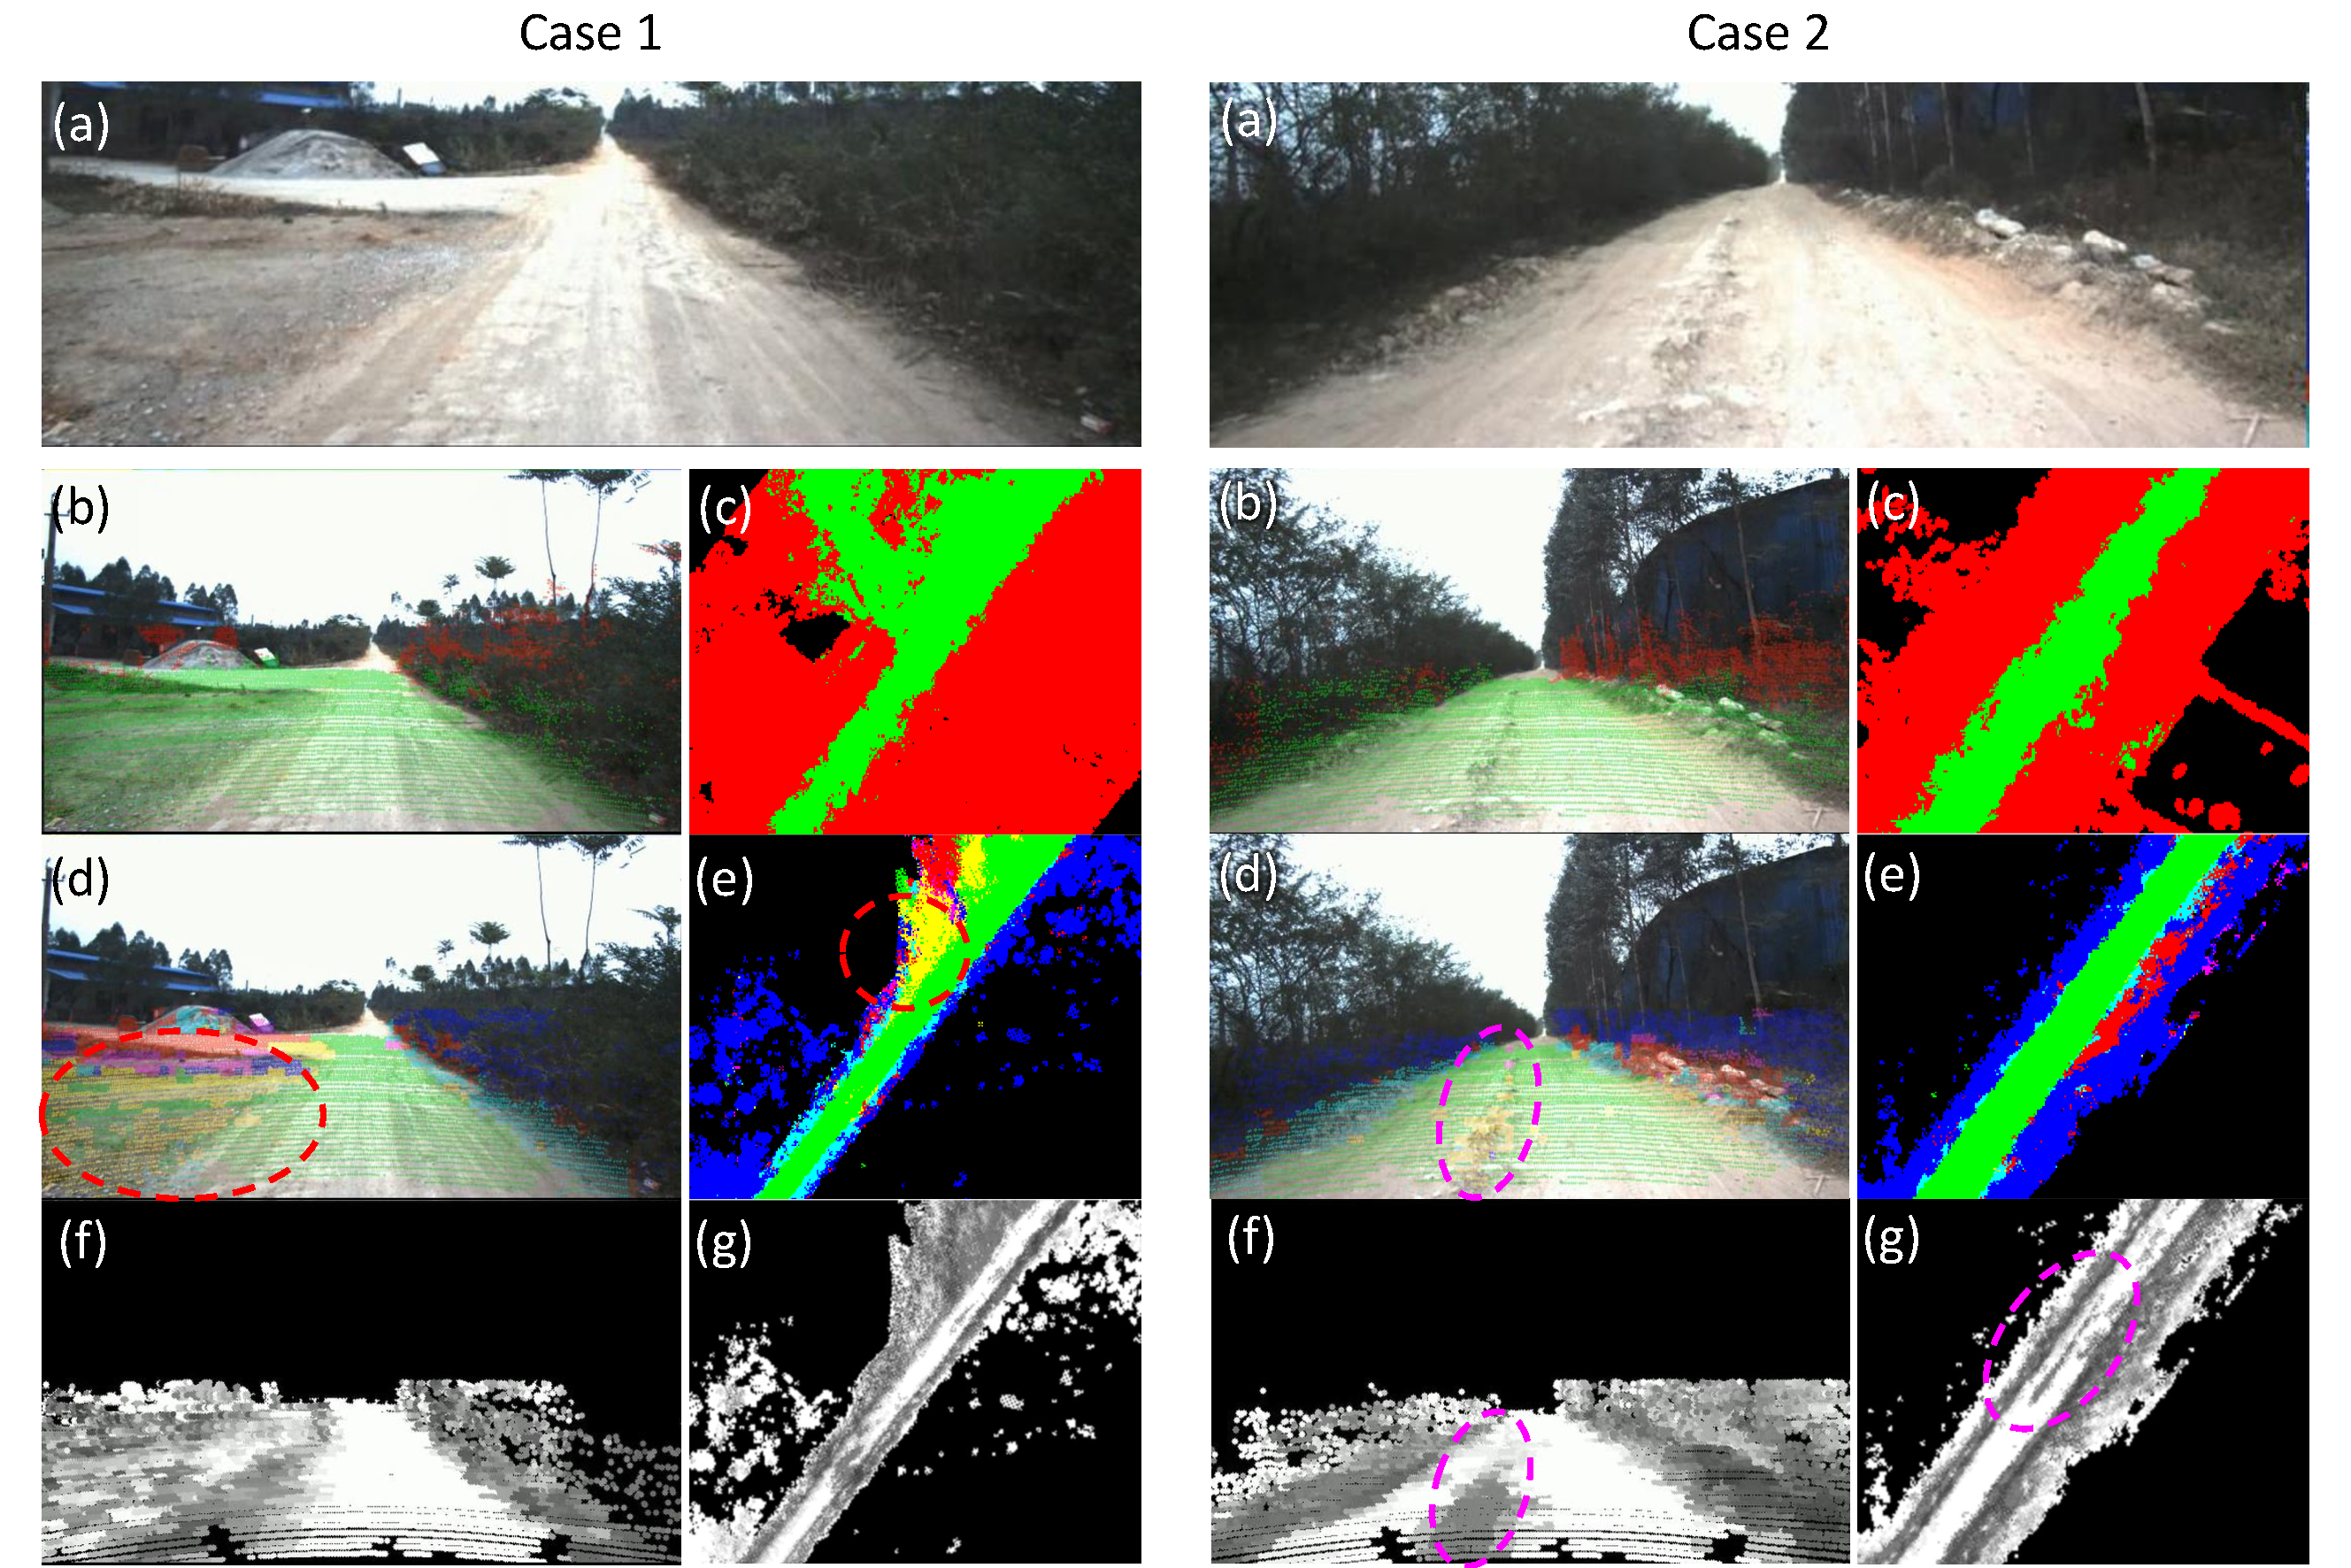
\includegraphics[width=0.85\textwidth]{semantic_mapping.pdf}
		\caption{Case study of fine-grained semantic map and confidence map, compared with coarse-grained  results. (a) scene image. (b) coarse-grained segmentation (binary classification). (c) coarse-grained semantic map (bird's-eye-view). (d) fine-grained semantic segmentation (projected on point clouds). (e) fine-grained semantic map (bird's-eye-view). (f) confidence map projected to camera-view, whiter pixels indicate higher confidence. (g) bird's-eye-view confidence map.}
		\label{fig:semantic_mapping}
		\vspace{-4mm}
	\end{figure*}
	
	To explore how clustering number $\mathcal{K}$ affects models' performance, an ablation study is made as shown in Fig.~\ref{fig:kmeans_exp}. We can find that the models' performance with regard to $\mathcal{K}$ are basically stable when $\mathcal{K} \geq 4$, and slightly decrease when $\mathcal{K}>6$. In general, models' performance approximately orders the same as Table~\ref{tab:cross_eval}. Therefore, we choose $\mathcal{K}=6$ as other experiments' setting to balance the fine-grained demand and model performance.
	
	\textbf{In summary, the proposed method achieves 89.8\% average anchor accuracy in cross-scene validation, and the performance is stable with regard to different clustering numbers, which demonstrates the robustness and generalization of our method.}
	
	
	\subsubsection{Fine-Grained Semantic Segmentation and Mapping}
	%1. 如图\ref{fig:semantic_segmentation}所示,展示了一些细粒度语义分割的结果;
	%2. 为了验证细粒度语义分割的实用性,我们构建了语义地图和置信度地图(简要介绍如何建图)。结合图\ref{fig:semantic_mapping}的case分析;
	%3. 借助激光雷达的数据,我们统计了各类别对应的激光点高度均值、方差的分布,结合图\ref{fig:lidar_analysis}进行说明;
	%结论:我们的算法能够的到有效的细粒度语义分割结果,并可以用于语义地图、场景理解等应用中。
	
	Due to the absence of pixel-level annotations for the task, we next demonstrate the validity of our fine-grained results through case studies and additional LiDAR data analysis. The following results are all based on the model trained by 50 frames of subset A.
	
	Fig.~\ref{fig:semantic_segmentation} shows some cases of fine-grained semantic segmentation. Because this work focuses on off-road traversability analysis, so only the bottom half of the image is predicted for simplicity. The semantic labels are not pre-designed, but we can find their intrinsic meanings through these concrete cases. For example, \textit{green} indicates hard earth road and paved road, \textit{blue} pixels are vegetation, \textit{yellow} pixels are road with fallen leaves or soft earth, \textit{red} pixels are stones or woods, etc. Different clusters can generally distinguish diverse semantic meanings.
	
	Statistical analysis is provided in Fig.~\ref{fig:lidar_analysis}, which is based on 3D LiDAR data with labels projected from image semantic segmentation.
	%By the way, semantic meanings of the color table are not pre-defined but concluded from our model's predictions.
	In Fig.~\ref{fig:lidar_analysis}(a-c), three categories' terrain elevation (\textit{green}, \textit{yellow}, and \textit{cyan}) mainly distribute around the ground level, which are three primary road types. Furthermore, from Fig.~\ref{fig:lidar_analysis}(d-f), we can find their different traversability cost. The \textit{green} boxes have the narrowest variance distribution, corresponding to the most easily passable paved road and hard earth. The \textit{yellow} and \textit{cyan} boxes are longer, indicating bumpier road surface. The \textit{blue} boxes indicate bushes and trees, with the highest elevation and traversability cost.
	\textbf{In a word, examined by associated 3D LiDAR data, the fine-grained segments of images are proved to have different levels of toughness and terrain elevation, which represents their semantical meaningfulness.}
	
	%To show the consistency of fine-grained predictions on continuous video frames and get overall scene understanding, we make semantic maps and confidence maps as described in Sec.~\ref{3_SM}. 
	The semantic maps and confidence maps are shown in Fig.~\ref{fig:semantic_mapping}. In case 1, our fine-grained predictions label the roadside area (\textit{yellow}) with higher traversability cost than middle road (\textit{green}). In case 2, bulges in the middle of the road are separated in the single frame segmentation, but not stable enough to obtain majority votes in the semantic map. The confidence map can be helpful to distinguish this subtle traversability difference, where the bumpy area is darker than other flat roads. \textbf{Therefore, the resultant fine-grained semantic maps and confidence maps can provide rich information for robots to traverse in complex off-road scenes.}
	
	\begin{figure*}[]
		\centering
		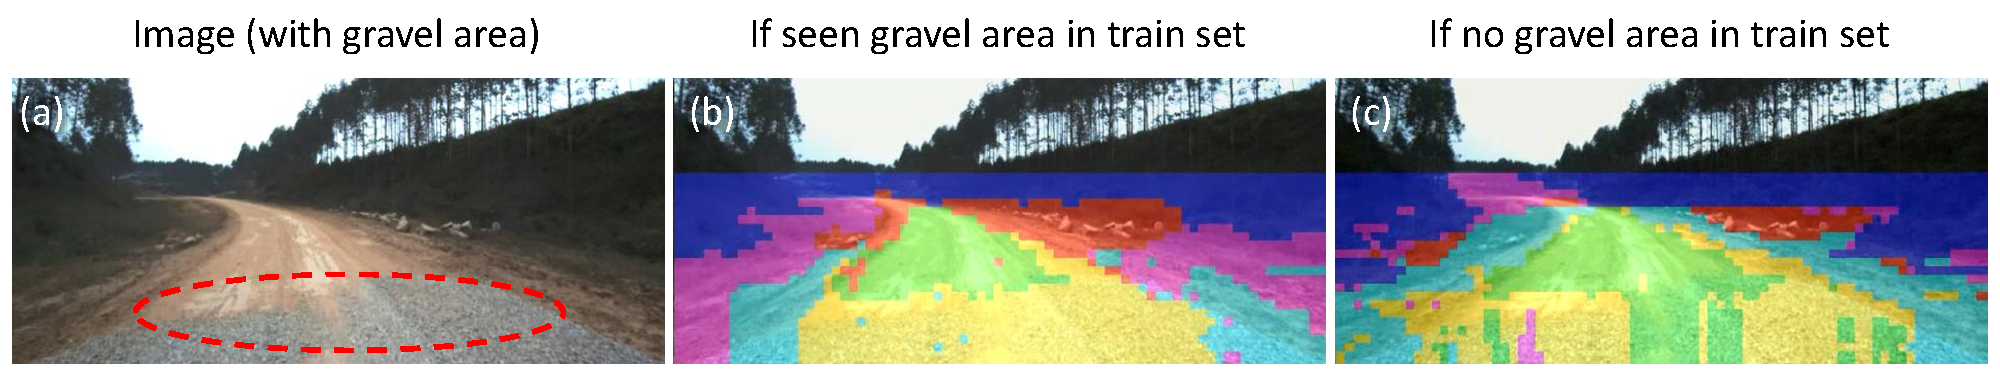
\includegraphics[width=0.85\textwidth]{challenges.pdf}
		\caption{A challenging case: when meeting unseen semantic categories.}
		\label{fig:challenges}
		\vspace{-4mm}
	\end{figure*}
	
	\subsection{Challenges}
	%1. 预测结果连续性不够好且计算复杂度高:目前添加背景引入上下文信息的方式比较简单,预测过程中滑动窗逐个预测patch类别,并没有显式地用到一致性先验;将来需要探究如何利用时空一致性优化性能和计算效率。
	%2. 没有见过的路面材质/OOD样本:目前的方法是根据K-Means结果强行并入某一类,将来需要进一步探究如何让算法主动发现OOD样本,并请求人工标注,使得模型可以增量式学习、更新。
	Currently, there are still some challenges with the proposed method. Firstly, the current pipeline to obtain dense predictions has a high computational cost. Predicting one image patch takes about 30 ms on an NVIDIA TITAN X. Although parallel computing helps to predict more patches at one time, the repetitive computation of overlapped patches can be optimized by temporal and spatial consistency in future works.
	The second one is unseen semantic categories, or called out of distribution (OOD) samples, as shown in Fig.~\ref{fig:challenges}. The current pipeline will not discriminate unseen category samples, but simply classified them into existing semantic clusters, which may lead to confused predictions as Fig.~\ref{fig:challenges}(c). To minimize labor costs, the OOD sample detection and incremental training mechanism deserve to be explored in our future works.
	
	
	
	\section{CONCLUSIONS}	\label{conclusions}
	In this paper, we propose a contrastive learning based method for off-road fine-grained semantic segmentation and mapping. With a set of human-annotated anchor patches, a feature representation is learned to discriminate regions with different traversability. After that, the fine-grained semantic segmentation and mapping pipeline is proposed for off-road scene understanding.
	For the experimental study of our method, we develop an off-road dataset with three driving segments that represent very diverse off-road scenes. The proposed method achieves 89.8\% anchor accuracy in cross-scene validation by evaluating the matching with human-annotated image patches.
	Examined by associated 3D LiDAR data, the fine-grained segments of visual images are demonstrated to have different levels of toughness and terrain elevation, which represents their semantical meaningfulness.
	The resultant maps contain both fine-grained labels and confidence values, providing rich information to support a robot traversing complex off-road scenes.
	%In this paper, we propose a fine-grained off-road semantic segmentation and mapping method based on contrastive learning techniques. 
	%The proposed method can learn discriminative feature representations with only a small number of sparse anchor annotations, with no demand for laborious pixel-level labels, which significantly reduces labeling difficulties and cost in off-road environments.
	%We examine our fine-grained results across diverse off-road scenes and prove its validity through additional LiDAR data analysis.
	Future work will be addressed on improving the computational efficiency by temporal and spatial consistency, and exploring OOD sample detection mechanism and incremental learning ability for long-term deployment on off-road robots.
	
	%\addtolength{\textheight}{-12cm}   % This command serves to balance the column lengths
	% on the last page of the document manually. It shortens
	% the textheight of the last page by a suitable amount.
	% This command does not take effect until the next page
	% so it should come on the page before the last. Make
	% sure that you do not shorten the textheight too much.
	
	%%%%%%%%%%%%%%%%%%%%%%%%%%%%%%%%%%%%%%%%%%%%%%%%%%%%%%%%%%%%%%%%%%%%%%%%%%%%%%%%
	
	
	
	%%%%%%%%%%%%%%%%%%%%%%%%%%%%%%%%%%%%%%%%%%%%%%%%%%%%%%%%%%%%%%%%%%%%%%%%%%%%%%%%
	
	
	
	%%%%%%%%%%%%%%%%%%%%%%%%%%%%%%%%%%%%%%%%%%%%%%%%%%%%%%%%%%%%%%%%%%%%%%%%%%%%%%%%
	%\section*{APPENDIX}
	
	%Appendixes should appear before the acknowledgment.
	
	%\section*{ACKNOWLEDGMENT}
	
	%The preferred spelling of the word ÒacknowledgmentÓ in America is without an ÒeÓ after the ÒgÓ. Avoid the stilted expression, ÒOne of us (R. B. G.) thanks . . .Ó  Instead, try ÒR. B. G. thanksÓ. Put sponsor acknowledgments in the unnumbered footnote on the first page.
	
	
	
	%%%%%%%%%%%%%%%%%%%%%%%%%%%%%%%%%%%%%%%%%%%%%%%%%%%%%%%%%%%%%%%%%%%%%%%%%%%%%%%%
	
	%References are important to the reader; therefore, each citation must be complete and correct. If at all possible, references should be commonly available publications.
	
	\printbibliography
	%\bibliographystyle{unsrt}
	%\bibliography{root}
	
	%\begin{thebibliography}{99}
	%
	%\bibitem{c1} G. O. Young, ÒSynthetic structure of industrial plastics (Book style with paper title and editor),Ó 	in Plastics, 2nd ed. vol. 3, J. Peters, Ed.  New York: McGraw-Hill, 1964, pp. 15Ð64.
	%
	%\end{thebibliography}
	
	
	
	
\end{document}
